
\section{Two Dimensional Plot Types}

{%
\tikzset{external/figure name/.add={}{twodim_}}

\PGFPlots{} supports several two-dimensional line plots like piecewise linear
line plots, piecewise constant plots, smoothed plots, bar plots and comb plots.
Most of them use the \PGF{} plot handler library directly, see
\cite[Section~18.8]{tikz}.

Plot types are part of the plot style, so they are set with options. Most of
the basic 2d plot types are part of \Tikz{}, see \cite[Section~18.8]{tikz}, and
are probably known to users of \Tikz{}. They are documented here as well.


\subsection{Linear Plots}

\begin{plottype}{sharp plot}
    Linear (`sharp') plots are the default. Point coordinates are simply
    connected by straight lines.
\begin{codeexample}[]
\begin{tikzpicture}
\begin{axis}
    \addplot+ [
        sharp plot,
    ] coordinates {
        (0,0) (1,2) (2,3)
    };
\end{axis}
\end{tikzpicture}
\end{codeexample}

    The `|+|' here means to use the normal plot cycle list and append
    `|sharp plot|' to its option list.
\end{plottype}


\subsection{Smooth Plots}

\begin{plottype}{smooth}
    Smooth plots interpolate smoothly between successive points.
\begin{codeexample}[]
\begin{tikzpicture}
\begin{axis}
    \addplot+ [
        smooth,
    ] coordinates {
        (0,0) (1,2) (2,3)
    };
\end{axis}
\end{tikzpicture}
\end{codeexample}
\end{plottype}

As described in~\cite{tikz} in all detail, this plot handler results in a
``smooth'' outline. However, it ``not very intelligent'' (compare~\cite{tikz})
and is unrelated to common plot-based interpolation schemes.

\begin{key}{/tikz/tension=\marg{tension} (initially 0.55)}
    A parameter which controls how the remaining degrees of freedom are fixed:
    it controls the smoothing effect. Higher values results in more ``rounded''
    corners whereas low values result in sharp corners.

    Please refer to~\cite{tikz} for details.
\end{key}


\subsection{Constant Plots}

Constant plots draw lines parallel to the $x$-axis to connect coordinates. The
discontinuous edges may be drawn or not, and marks may be placed on left or
right ends.

\begin{plottype}{const plot}
    Connects all points with horizontal and vertical lines. Marks are placed
    left-handed on horizontal line segments, causing the plot to be right-sided
    continuous at all data points.

\begin{codeexample}[]
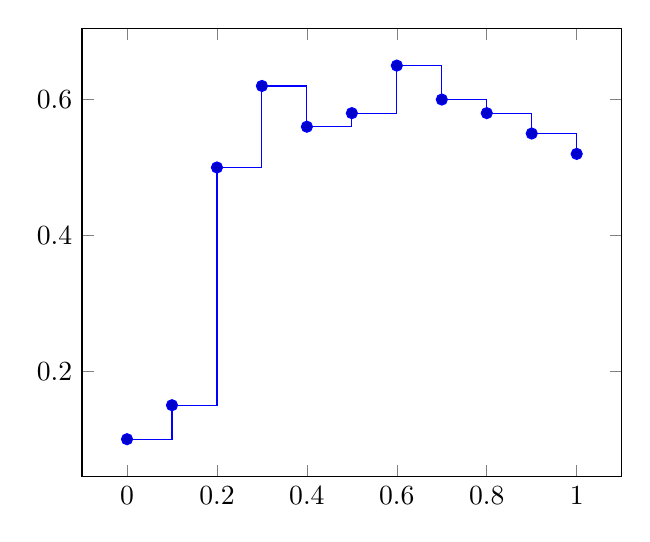
\begin{tikzpicture}
\begin{axis}
    \addplot+ [
        const plot,
    ] coordinates {
        (0,0.1)    (0.1,0.15)  (0.2,0.5)   (0.3,0.62)
        (0.4,0.56) (0.5,0.58)  (0.6,0.65)  (0.7,0.6)
        (0.8,0.58) (0.9,0.55)  (1,0.52)
    };
\end{axis}
\end{tikzpicture}
\end{codeexample}


\begin{codeexample}[]
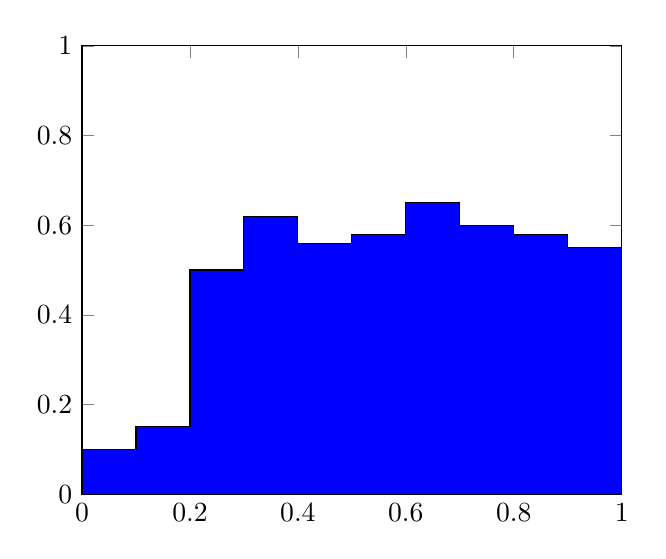
\begin{tikzpicture}
\begin{axis}[ymin=0,ymax=1,enlargelimits=false]
    \addplot [
        const plot,
        fill=blue,
        draw=black,
    ] coordinates {
        (0,0.1)    (0.1,0.15)  (0.2,0.5)   (0.3,0.62)
        (0.4,0.56) (0.5,0.58)  (0.6,0.65)  (0.7,0.6)
        (0.8,0.58) (0.9,0.55)  (1,0.52)
    }
        \closedcycle
    ;
\end{axis}
\end{tikzpicture}
\end{codeexample}
\end{plottype}

\begin{plottype}{const plot mark left}
    An alias for `|const plot|'.
\end{plottype}

\begin{plottype}{const plot mark right}
    A variant which places marks on the right of each line segment, causing
    plots to be left-sided continuous at the given coordinates.
    %
\begin{codeexample}[]
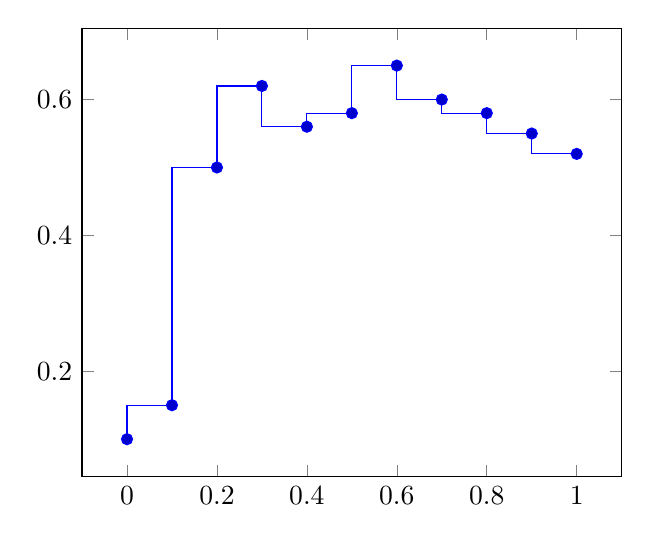
\begin{tikzpicture}
\begin{axis}
    \addplot+ [
        const plot mark right,
    ] coordinates {
        (0,0.1)    (0.1,0.15)  (0.2,0.5)   (0.3,0.62)
        (0.4,0.56) (0.5,0.58)  (0.6,0.65)  (0.7,0.6)
        (0.8,0.58) (0.9,0.55)  (1,0.52)
    };
\end{axis}
\end{tikzpicture}
\end{codeexample}
\end{plottype}

\begin{plottype}{const plot mark mid}
    A variant which places marks in the middle of each line segment, causing
    plots to be symmetric around its data points.
    %
\begin{codeexample}[]
\begin{tikzpicture}
\begin{axis}
    \addplot+ [
        const plot mark mid,
    ] coordinates {
        (0,0.1)    (0.1,0.15)  (0.2,0.5)   (0.3,0.62)
        (0.4,0.56) (0.5,0.58)  (0.6,0.65)  (0.7,0.6)
        (0.8,0.58) (0.9,0.55)  (1,0.52)
    };
\end{axis}
\end{tikzpicture}
\end{codeexample}
    %
    Note that ``symmetric'' is only true for constant mesh width: if the
    $x$-distances between adjacent data points differ, |const plot mark mid|
    will produce vertical lines in the middle between each pair of consecutive
    points.
\end{plottype}

\begin{plottype}{jump mark left}
    A variant of `|const plot mark left|' which does not draw vertical lines.
    %
\begin{codeexample}[]
\begin{tikzpicture}
\begin{axis}[samples=8]
    \addplot+ [
        jump mark left,
        domain=-5:0,
    ] {4*x^2 - 5};

    \addplot+ [
        jump mark right,
        domain=-5:0,
    ] {0.7*x^3 + 50};
\end{axis}
\end{tikzpicture}
\end{codeexample}
\end{plottype}

\begin{plottype}{jump mark right}
    A variant of `|const plot mark right|' which does not draw vertical lines.
\end{plottype}

\begin{plottype}{jump mark mid}
    A variant of `|const plot mark mid|' which does not draw vertical lines.
    %
\begin{codeexample}[]
\begin{tikzpicture}
\begin{axis}
    \addplot+ [
        jump mark mid,
    ] coordinates {
        (0,0.1)    (0.1,0.15)  (0.2,0.5)   (0.3,0.62)
        (0.4,0.56) (0.5,0.58)  (0.6,0.65)  (0.7,0.6)
        (0.8,0.58) (0.9,0.55)  (1,0.52)
    };
\end{axis}
\end{tikzpicture}
\end{codeexample}
\end{plottype}


\subsection{Bar Plots}

Bar plots place horizontal or vertical bars at coordinates. Multiple bar plots
in one axis can be stacked on top of each other or aligned next to each other.

\begin{plottype}{xbar}
    Places horizontal bars between the $(y=0)$ line and each coordinate.

    This option is used on a per-plot basis and configures only the
    visualization of coordinates. The figure-wide style |/pgfplots/xbar| also
    sets reasonable options for ticks, legends and multiple plots.
    %
\begin{codeexample}[]
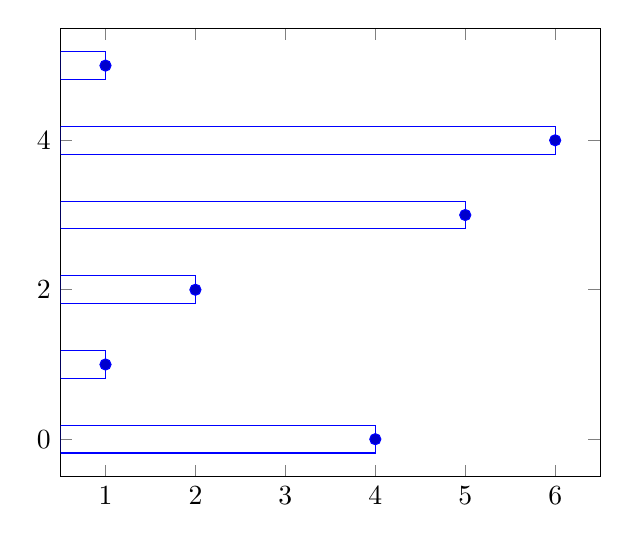
\begin{tikzpicture}
\begin{axis}
    \addplot+ [
        xbar,
    ] coordinates {
        (4,0) (1,1) (2,2)
        (5,3) (6,4) (1,5)
    };
\end{axis}
\end{tikzpicture}
\end{codeexample}
    %
    Bars are centered at plot coordinates with width |bar width|. Using bar
    plots usually means more than just a different way of how to connect
    coordinates, for example to draw ticks outside of the axis, change the
    legend's appearance or introduce shifts if multiple |\addplot| commands
    appear.

    There is a pre-configured style for |xbar| which is installed automatically
    if you provide |xbar| as argument to the axis environment which provides
    this functionality.
    %
% \usetikzlibrary{patterns}
\begin{codeexample}[]
\begin{tikzpicture}
\begin{axis}[xbar,enlargelimits=0.15]
    \addplot [draw=blue,
        pattern=horizontal lines light blue,
    ] coordinates {
        (10,5) (15,10) (5,15) (24,20) (30,25)
    };
    \addplot [draw=black,
        pattern=horizontal lines dark blue,
    ] coordinates {
        (3,5) (5,10) (15,15) (20,20) (35,25)
    };
\end{axis}
\end{tikzpicture}
\end{codeexample}
    %
    Here |xbar| yields |/pgfplots/xbar| because it is an argument to the axis,
    not to a single plot.

    For bar plots, it is quite common to provide textual coordinates or even
    descriptive nodes near the bars. This can be implemented using the keys
    |symbolic y coords| and |nodes near coords|, respectively:
    %
\begin{codeexample}[]
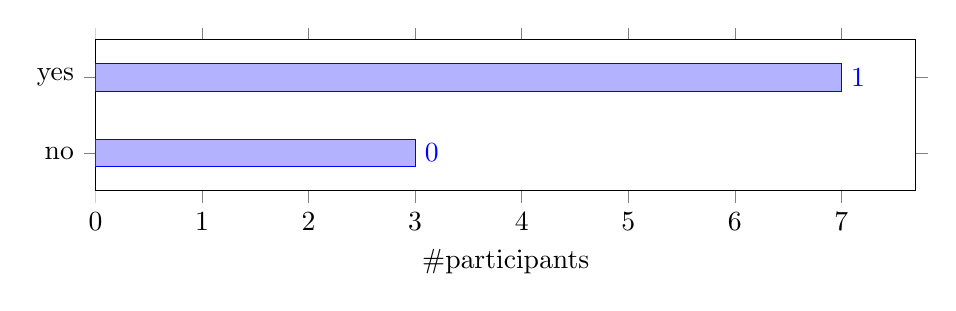
\begin{tikzpicture}
    \begin{axis}[
        xbar, xmin=0,
        width=12cm, height=3.5cm, enlarge y limits=0.5,
        xlabel={\#participants},
        symbolic y coords={no,yes},
        ytick=data,
        nodes near coords, nodes near coords align={horizontal},
    ]
        \addplot coordinates {(3,no) (7,yes)};
    \end{axis}
\end{tikzpicture}
\end{codeexample}
    %
    The |symbolic y coords| defines a dictionary of accepted coordinates which
    are then expected in $y$-coordinates and the |nodes near coords| key
    displays values as extra nodes (see their reference documentations for
    details). The example employs |enlarge y limits| in order to get some more
    free space since the default spacing is not always appropriate for bar
    plots.

    Note that it might be quite important to include |xmin=0| explicitly as in
    the example above. Without it, the lower bound will be used:
    %
\begin{codeexample}[]
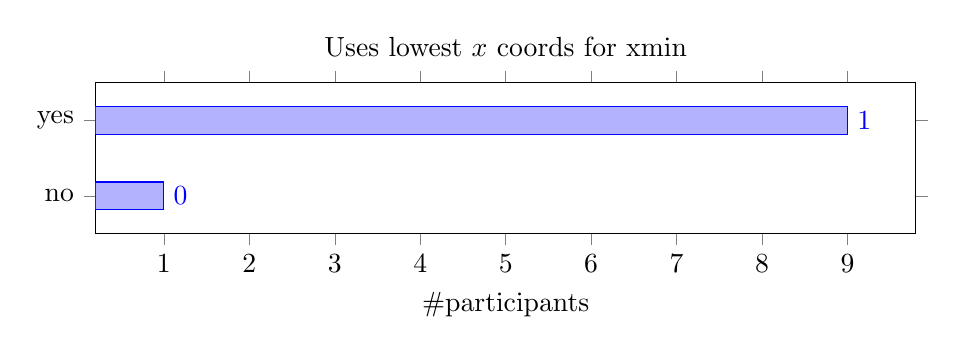
\begin{tikzpicture}
    \begin{axis}[
        title=Uses lowest $x$ coords for xmin,
        xbar,
        width=12cm, height=3.5cm, enlarge y limits=0.5,
        xlabel={\#participants},
        symbolic y coords={no,yes},
        ytick=data,
        nodes near coords, nodes near coords align={horizontal},
      ]
        \addplot coordinates {(1,no) (9,yes)};
    \end{axis}
\end{tikzpicture}
\end{codeexample}

    Besides line, fill, and color styles, bars can be configured with
    |bar width| and |bar shift|, see below.
\end{plottype}

\begin{stylekey}{/pgfplots/xbar=\marg{shift for multiple plots} (default 2pt)}
    This style sets |/tikz/xbar| \emph{and} some commonly used options
    concerning horizontal bars for the complete axis. This is automatically
    done if you provide |xbar| as argument to an axis argument, see above.

    The |xbar| style defines shifts if multiple plots are placed into one axis.
    It draws bars adjacent to each other, separated by \meta{shift for multiple
    plots}. Furthermore, it sets the style |bar cycle list| and sets tick and
    legend appearance options.

    The style is defined as follows.
    %
\begin{codeexample}[code only]
\pgfplotsset{
    /pgfplots/xbar/.style={
        /tikz/xbar,
        bar cycle list,
        tick align=outside,
        xbar legend,
        /pgfplots/bar shift auto={#1},
    },
}
\end{codeexample}

    \begin{pgfplotskey}{bar shift auto=\marg{shift for multiple plots} (default 2pt)}
        The formula for |bar shift| assigns shifts dependent on the total
        number of plots and the current plot's number. It is designed to fill a
        total width of $n \cdot $|bar width|$ + (n-1) \cdot $\meta{shift for
        multiple plots}. The $0.5$ compensates for centering.

        The style is defined as
        %
\begin{codeexample}[code only]
\pgfplotsset{
    /pgfplots/bar shift auto/.style={
        /pgf/bar shift={%
            % total width = n*w + (n-1)*skip
            % -> subtract half for centering
            -0.5*(\numplotsofactualtype*\pgfplotbarwidth + (\numplotsofactualtype-1)*(#1)) +
            % the '0.5*w' is for centering
            (.5+\plotnumofactualtype)*\pgfplotbarwidth + \plotnumofactualtype*(#1)},
    },
}
\end{codeexample}
    \end{pgfplotskey}
\end{stylekey}

\begin{plottype}{ybar}
    Like |xbar|, this option generates bar plots. It draws vertical bars
    between the ($x=0$) line and each input coordinate.
    %
\begin{codeexample}[]
\begin{tikzpicture}
\begin{axis}
    \addplot+ [
        ybar,
    ] coordinates {
        (0,3) (1,2) (2,4) (3,1) (4,2)
    };
\end{axis}
\end{tikzpicture}
\end{codeexample}
    %
    The example above simply changes how input coordinates shall be visualized.
    As mentioned for |xbar|, one usually needs modified legends and shifts for
    multiple bars in the same axis.

    There is a predefined style which installs these customizations when
    provided to the axis environment:
    %
\begin{codeexample}[]
\begin{tikzpicture}
\begin{axis}[
    x tick label style={
        /pgf/number format/1000 sep=},
    ylabel=Population,
    enlargelimits=0.15,
    legend style={at={(0.5,-0.15)},
        anchor=north,legend columns=-1},
    ybar,
    bar width=7pt,
]
    \addplot coordinates {
        (1930,50e6) (1940,33e6)
        (1950,40e6) (1960,50e6) (1970,70e6)
    };
    \addplot coordinates {
        (1930,38e6) (1940,42e6)
        (1950,43e6) (1960,45e6) (1970,65e6)
    };
    \addplot coordinates {
        (1930,15e6) (1940,12e6)
        (1950,13e6) (1960,25e6) (1970,35e6)
    };
    \addplot [red,line legend,
        sharp plot,update limits=false,
    ] coordinates { (1910,4.3e7) (1990,4.3e7) }
        node [above] at (1950,4.3e7) {Houses};

    \legend{Far,Near,Here,Annot}
\end{axis}
\end{tikzpicture}
\end{codeexample}
    %
    Here, |ybar| yields |/pgfplots/ybar| because it is an argument to the axis,
    not to a single plot. The style affects the first three |\addplot|
    commands. Note that it shifts them horizontally around the plot
    coordinates. The fourth |\addplot| command is some kind of annotation which
    doesn't |update limits|.

    The |ybar| style can be combined with |symbolic x coords| in a similar way
    as described for |xbar|:
    %
\begin{codeexample}[]
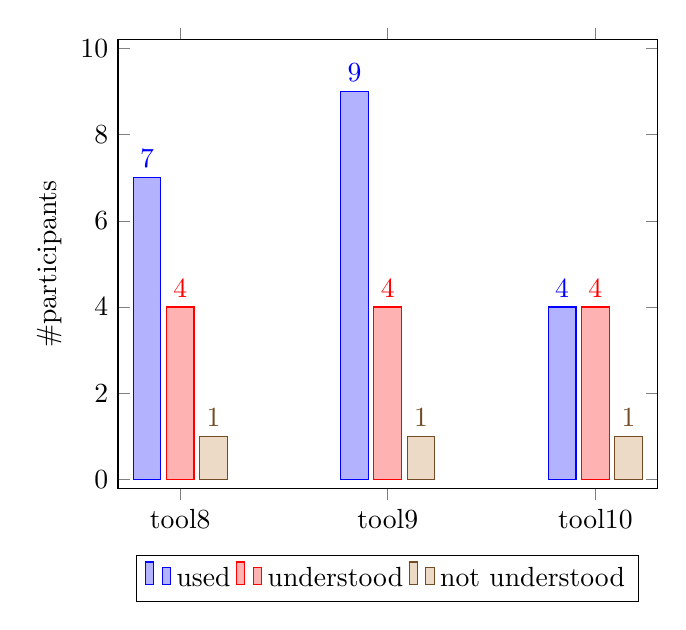
\begin{tikzpicture}
\begin{axis}[
    ybar,
    enlargelimits=0.15,
    legend style={at={(0.5,-0.15)},
    anchor=north,legend columns=-1},
    ylabel={\#participants},
    symbolic x coords={tool8,tool9,tool10},
    xtick=data,
    nodes near coords,
    nodes near coords align={vertical},
]
\addplot coordinates {(tool8,7) (tool9,9) (tool10,4)};
\addplot coordinates {(tool8,4) (tool9,4) (tool10,4)};
\addplot coordinates {(tool8,1) (tool9,1) (tool10,1)};
    \legend{used,understood,not understood}
\end{axis}
\end{tikzpicture}
\end{codeexample}

    As for |xbar|, the bar width and shift can be configured with |bar width|
    and |bar shift|. However, the bar shift is better provided as argument to
    |/pgfplots/ybar| since this style will overwrite the bar shift. Thus,
    prefer |/pgfplots/ybar=4pt| to set the bar shift.

    Sometimes it is useful to write the $y$ values directly near the bars. This
    can be realized using the |nodes near coords| method:
    %
\begin{codeexample}[]
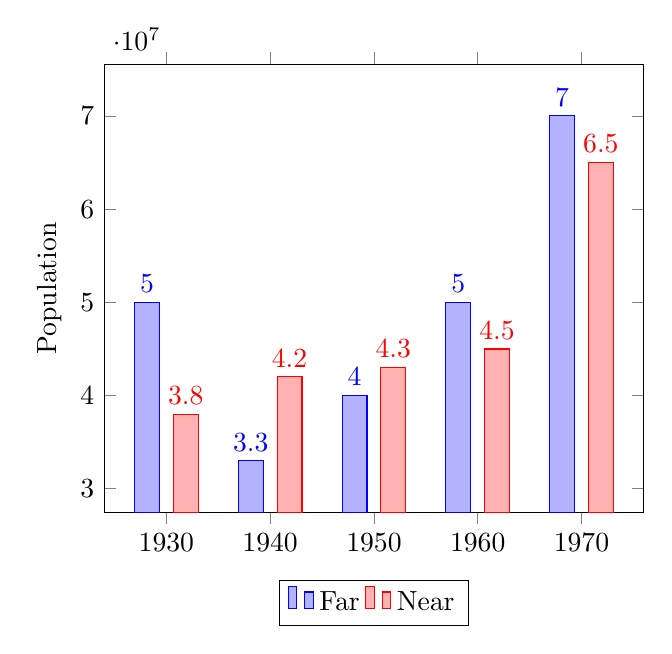
\begin{tikzpicture}
\begin{axis}[
    x tick label style={
        /pgf/number format/1000 sep=},
    ylabel=Population,
    enlargelimits=0.15,
    legend style={at={(0.5,-0.15)},
        anchor=north,legend columns=-1},
    ybar=5pt,% configures `bar shift'
    bar width=9pt,
    nodes near coords,
    point meta=y *10^-7, % the displayed number
]
    \addplot coordinates {
        (1930,50e6) (1940,33e6)
        (1950,40e6) (1960,50e6) (1970,70e6)
    };
    \addplot coordinates {
        (1930,38e6) (1940,42e6)
        (1950,43e6) (1960,45e6) (1970,65e6)
    };
    \legend{Far,Near}
\end{axis}
\end{tikzpicture}
\end{codeexample}

    Any support style changes are possible, of course. A useful example for bar
    plots might be to use rotated tick labels:
    %
\begin{codeexample}[]
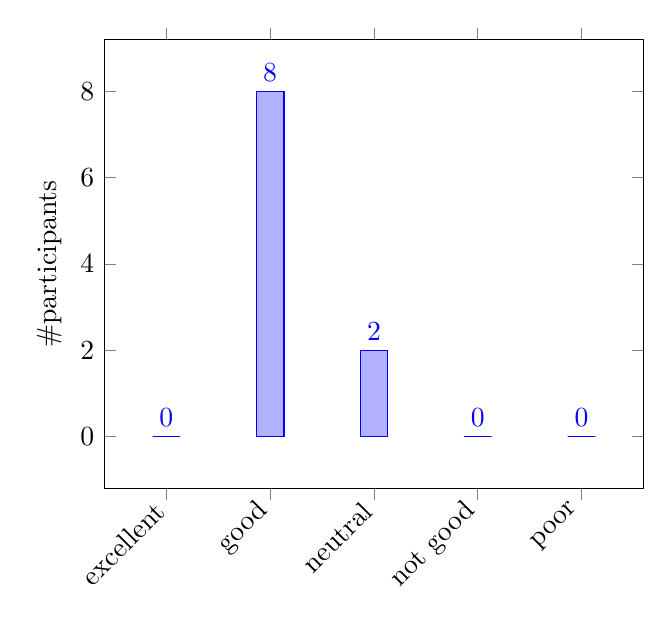
\begin{tikzpicture}
\begin{axis}[
    ybar,
    enlargelimits=0.15,
    legend style={at={(0.5,-0.2)},
    anchor=north,legend columns=-1},
    ylabel={\#participants},
    symbolic x coords={excellent,good,neutral,%
        not good,poor},
    xtick=data,
    nodes near coords,
    nodes near coords align={vertical},
    x tick label style={rotate=45,anchor=east},
]
    \addplot coordinates {
        (excellent,0) (good,8) (neutral,2)
        (not good,0) (poor,0)
    };
\end{axis}
\end{tikzpicture}
\end{codeexample}
\end{plottype}

\begin{stylekey}{/pgfplots/ybar=\marg{shift for multiple plots} (default 2pt)}
    As |/pgfplots/xbar|, this style sets the |/tikz/ybar| option to draw
    vertical bars, but it also provides commonly used options for vertical
    bars.

    If you supply |ybar| to an axis environment, |/pgfplots/ybar| will be
    chosen instead of |/tikz/ybar|.

    It changes the legend, draws ticks outside of the axis lines and draws
    multiple |\addplot| arguments adjacent to each other; block-centered at the
    $x$-coordinate and separated by \meta{shift for multiple plots}. It will
    also install the |bar shift| for |every node near coord|. Furthermore, it
    installs the style |bar cycle list|. It is defined similarly to
    |/pgfplots/xbar|.
\end{stylekey}

\begin{pgfplotskey}{bar cycle list}
    A style which installs cycle lists for multiple bar plots.
    %
\begin{codeexample}[code only]
\pgfplotsset{
    /pgfplots/bar cycle list/.style={/pgfplots/cycle list={
            {blue,fill=blue!30!white,mark=none},
            {red,fill=red!30!white,mark=none},
            {brown!60!black,fill=brown!30!white,mark=none},
            {black,fill=gray,mark=none},
        },
    },
}
\end{codeexample}
\end{pgfplotskey}

\begin{key}{/pgf/bar width=\marg{dimension or unit} (initially 10pt)}
    Configures the width used by |xbar| and |ybar|. It is accepted to provide
    mathematical expressions.

    As of \PGFPlots{} 1.7, it is allows to provide a \emph{unit} as
    |bar width|. In this case, the |bar width| will be interpreted as axis unit:
    %
\begin{codeexample}[]
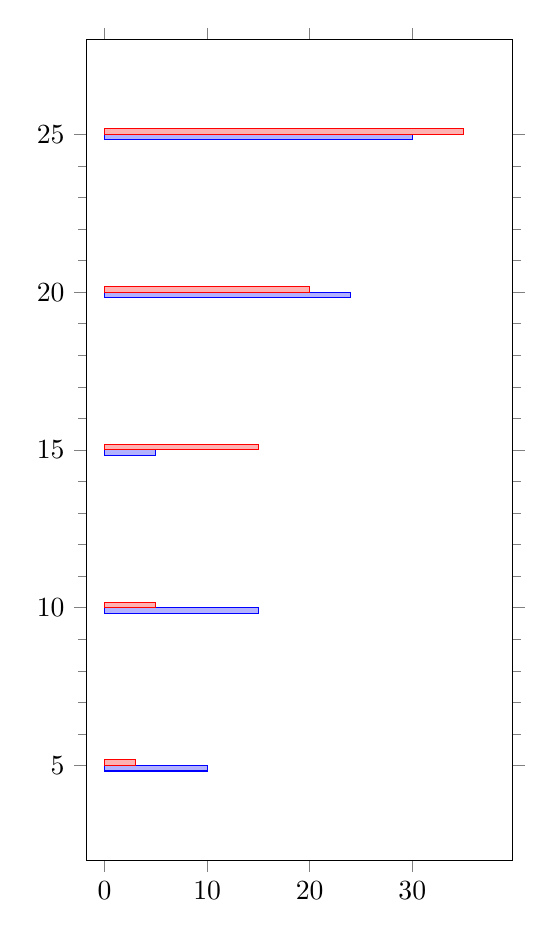
\begin{tikzpicture}
\begin{axis}[
    xbar=0pt,% space of 0pt between adjacent bars
    bar width=2,
    width=7cm,
    height=12cm,
    minor y tick num=4,
    ytick=data,
    enlargelimits=0.15,
]
    \addplot coordinates {
        (10,5) (15,10) (5,15) (24,20) (30,25)
    };
    \addplot coordinates {
        (3,5) (5,10) (15,15) (20,20) (35,25)
    };
\end{axis}
\end{tikzpicture}
\end{codeexample}
    %
    In order to interpret arguments as units, you have to write
    |\pgfplotsset{compat=1.7}| (or newer) into your preamble. Older versions
    will implicitly append the |pt| suffix if the argument is no dimension.

    \begin{command}{\pgfplotbarwidth}
        A mathematical expression which results in the fully computed value of
        |bar width| (i.e.\@ it includes any unit computations).
    \end{command}

    Note that you may need to |enlargelimits| in order to see the complete bar
    -- \PGFPlots{} will not automatically update the axis limits to respect
    |bar width|.
\end{key}

\begin{key}{/pgf/bar shift=\marg{dimension or unit} (initially 0pt)}
    Configures a shift for |xbar| and |ybar|. Use |bar shift| together with
    |bar width| to draw multiple bar plots into the same axis. It is accepted
    to provide mathematical expressions.

    As of \PGFPlots{}~1.7, it is allows to provide an \emph{unit} as
    |bar shift|. In this case, the |bar shift| will be interpreted as axis unit.

    \begin{command}{\pgfplotbarshift}
        A mathematical expression which results in the fully computed value of
        |bar shift| (i.e.\@ it includes any unit computations).
    \end{command}

    Note that you may need to |enlargelimits| in order to see the complete bar
    -- \PGFPlots{} will not automatically update the axis limits to respect
    |bar shift|.
\end{key}

\begin{pgfplotskey}{bar direction=\mchoice{auto,x,y} (initially auto)}
    If \PGFPlots{} encounters a value |bar width=1| (i.e.\@ \emph{without}
    dimension like |1pt|), it attempts to evaluate the bar's direction.

    The default configuration \declareandlabel{auto} assumes that you write
    something like |ybar,bar width=1|. In this case, it is clear that you have
    a $y$ bar and \PGFPlots{} assumes |bar direction=y|.

    However, this context information is unavailable. In this case, you can use
    the choice \declaretext{x} if \PGFPlots{} in unaware that it works on an
    |xbar| plot or \declaretext{y} if \PGFPlots{} is unaware that you meant an
    |ybar| plot.
\end{pgfplotskey}

\begin{plottype}{ybar interval}
    This plot type produces vertical bars with width (and shift) relatively to
    intervals of coordinates.

    There is one conceptional difference when working with intervals: an
    interval is defined by \emph{two} coordinates. Since |ybar| has one value
    for each interval, the $i$th bar is defined by
    %
    \begin{enumerate}
        \item the $y$ value of the $i$th coordinates,
        \item the $x$ value of the $i$th coordinate as left interval
            boundary,
        \item the $x$ value of the $(i+1)$th coordinate as right interval
            boundary.
    \end{enumerate}
    %
    Consequently, there is \emph{one coordinate too much}: the last coordinate
    will \emph{only} be used to determine the interval width; its $y$ value
    doesn't influence the bar appearance.

    It is installed on a per-plot basis and configures \emph{only} the
    visualization of coordinates. See the style |/pgfplots/ybar interval| which
    configures the appearance of the complete figure.
    %
\begin{codeexample}[]
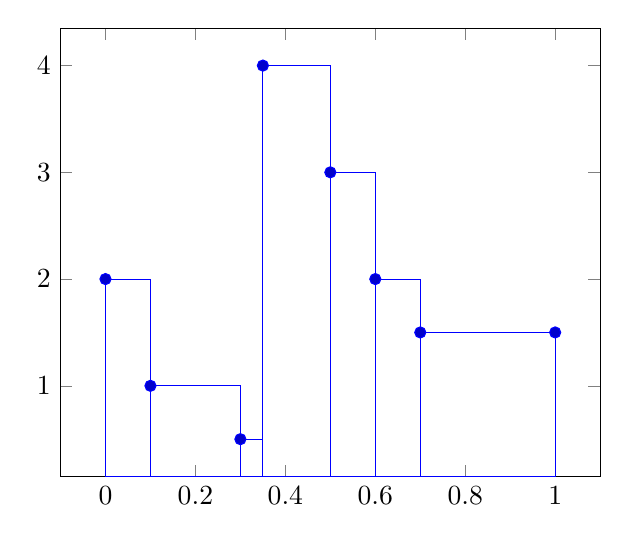
\begin{tikzpicture}
\begin{axis}
    \addplot+ [
        ybar interval,
    ] coordinates {
        (0,2) (0.1,1) (0.3,0.5) (0.35,4) (0.5,3)
        (0.6,2) (0.7,1.5) (1,1.5)
    };
\end{axis}
\end{tikzpicture}
\end{codeexample}

\begin{codeexample}[]
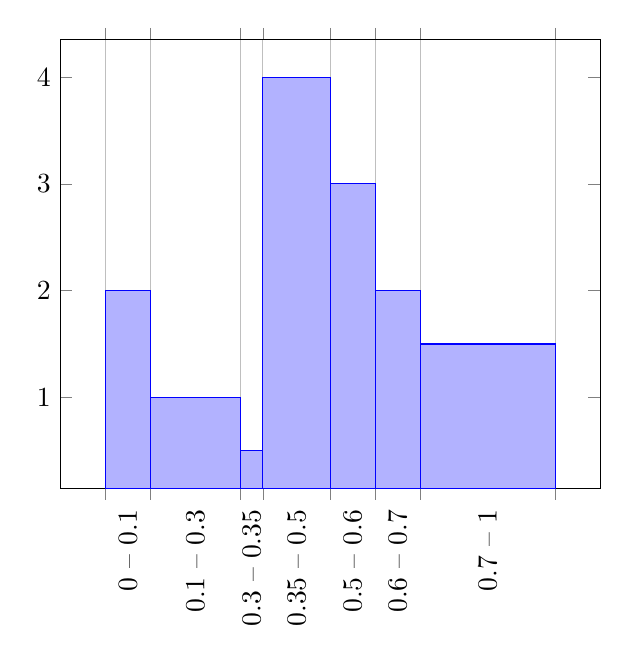
\begin{tikzpicture}
\begin{axis}[ybar interval,
    xtick=data,
    xticklabel interval boundaries,
    x tick label style={
        rotate=90,
        anchor=east,
    },
]
    \addplot coordinates {
        (0,2) (0.1,1) (0.3,0.5) (0.35,4) (0.5,3)
        (0.6,2) (0.7,1.5) (1,1.5)
    };
\end{axis}
\end{tikzpicture}
\end{codeexample}

\begin{codeexample}[]
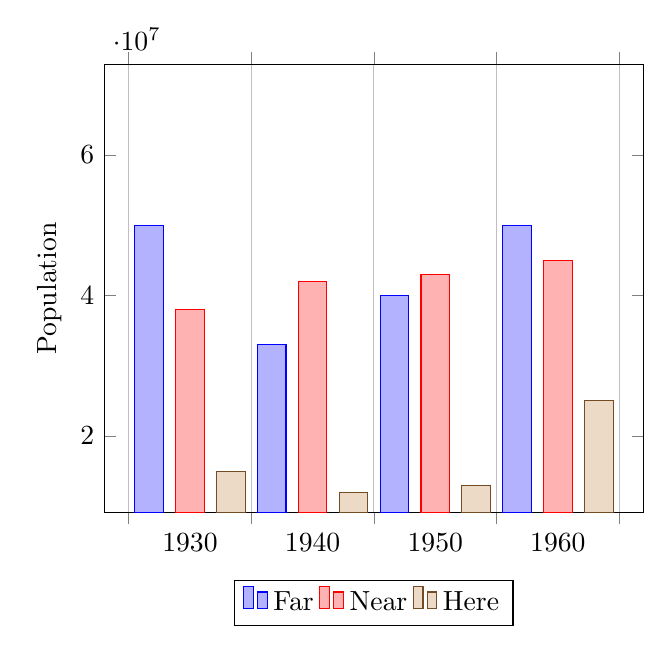
\begin{tikzpicture}
\begin{axis}[
    x tick label style={
        /pgf/number format/1000 sep=},
    ylabel=Population,
    enlargelimits=0.05,
    legend style={at={(0.5,-0.15)},
    anchor=north,legend columns=-1},
    ybar interval=0.7,
]
    \addplot coordinates {
        (1930,50e6) (1940,33e6)
        (1950,40e6) (1960,50e6) (1970,70e6)
    };
    \addplot coordinates {
        (1930,38e6) (1940,42e6)
        (1950,43e6) (1960,45e6) (1970,65e6)
    };
    \addplot coordinates {
        (1930,15e6) (1940,12e6)
        (1950,13e6) (1960,25e6) (1970,35e6)
    };
    \legend{Far,Near,Here}
\end{axis}
\end{tikzpicture}
\end{codeexample}
\end{plottype}

\begin{stylekey}{/pgfplots/ybar interval=\marg{relative width} (default 1)}
    A style which is intended to install options for |ybar interval| for a
    complete figure. This includes tick and legend appearance, management of
    multiple bar plots in one figure and a more adequate |cycle list| using the
    style |bar cycle list|.
\end{stylekey}

\begin{plottype}{xbar interval}
    As |ybar interval|, just for horizontal bars.
    %
\begin{codeexample}[]
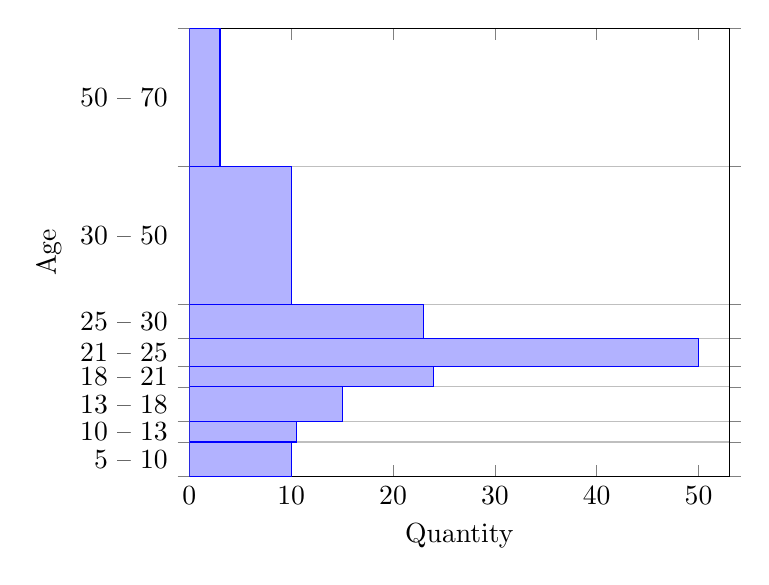
\begin{tikzpicture}
\begin{axis}[
    xmin=0,xmax=53,
    ylabel=Age,
    xlabel=Quantity,
    enlargelimits=false,
    ytick=data,
    yticklabel interval boundaries,
    xbar interval,
]
    \addplot coordinates {
        (10,5) (10.5,10) (15,13) (24,18) (50,21)
        (23,25) (10,30) (3,50) (3,70)
    };
\end{axis}
\end{tikzpicture}
\end{codeexample}
\end{plottype}

\begin{stylekey}{/pgfplots/xbar interval=\marg{relative width} (default 1)}
    A style which is intended to install options for |xbar interval| for a
    complete figure, see the style |/pgfplots/ybar interval| for details.
\end{stylekey}

\begin{pgfplotsxykey}{\x ticklabel interval boundaries}
    These are style keys which set |x tick label as interval| (see
    page~\pageref{key:pgfplots:ticklabelasinterval} for details) and configure
    the tick appearance to be \meta{start} -- \meta{end} for each tick
    interval.
\end{pgfplotsxykey}


\subsection{Histograms}

This section has been moved to the |statistics| library, see
Section~\ref{sec:histograms} on page~\pageref{sec:histograms}.


\subsection{Box Plots}

This section has been moved to the |statistics| library, see
Section~\ref{sec:boxplots} on page~\pageref{sec:boxplots}.


\subsection{Comb Plots}

Comb plots are very similar to bar plots except that they employ single
horizontal/vertical lines instead of rectangles.

\begin{plottype}{xcomb}
\begin{codeexample}[]
\begin{tikzpicture}
\begin{axis}
    \addplot+ [
        xcomb,
    ] coordinates {
        (4,0) (1,1) (2,2)
        (5,3) (6,4) (1,5)
    };
\end{axis}
\end{tikzpicture}
\end{codeexample}
\end{plottype}

\begin{plottype}{ycomb}
\begin{codeexample}[]
\begin{tikzpicture}
\begin{axis}
    \addplot+ [
        ycomb,
    ] coordinates {
        (0,3) (1,2) (2,4) (3,1) (4,2)
    };
\end{axis}
\end{tikzpicture}
\end{codeexample}
\end{plottype}


\subsection{Quiver Plots (Arrows)}
\label{sec:pgfplots:quiver2d}

\begin{plottype}[/pgfplots]{quiver=%
    \textcolor{black}{\marg{{\normalfont options with `\texttt{quiver/}' prefix}}}%
}
    A plot type which draws small arrows, starting at $(x,y)$, in direction of
    $(u,v)$.
    %
\begin{codeexample}[]
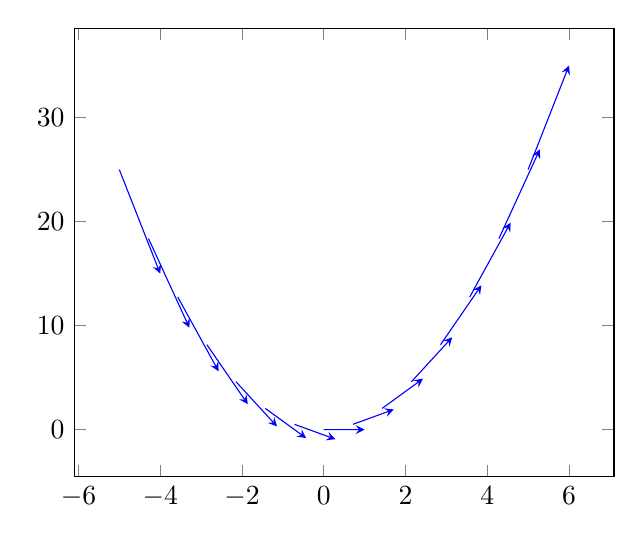
\begin{tikzpicture}
\begin{axis}
    \addplot [
        blue,
        quiver={u=1,v=2*x},
        -stealth,
        samples=15,
    ] {x^2};
\end{axis}
\end{tikzpicture}
\end{codeexample}

    The base point $(x,y)$ is provided as before; in the example above, it is
    generated by |\addplot expression| and yields $(x,x^2)$. The vector direction
    $(u,v)$ needs to be given in addition. Our example with |quiver/u=1| and
    |quiver/v=2*x| results in $u=1$ and $v=2x$. Thus, we have defined and
    visualized a vector field for the derivative of $f(x) = x^2$.

    A common example is to visualize the gradient $(\partial_x f,\partial_y
    f)(x,y)$ of a two-dimensional function $f(x,y)$:
    %
\pgfplotsexpensiveexample
\begin{codeexample}[]
\begin{tikzpicture}
\begin{axis}[
    title={$x \exp(-x^2-y^2)$ and its gradient},
    domain=-2:2,
    view={0}{90},
    axis background/.style={fill=white},
]
    \addplot3 [
        contour lua={number=9,labels=false},thick,
            ] {exp(0-x^2-y^2)*x};
    \addplot3 [
        blue,-stealth,samples=15,
        quiver={
            u={exp(0-x^2-y^2)*(1-2*x^2)},
            v={exp(0-x^2-y^2)*(-2*x*y)},
            scale arrows=0.3,
        },
    ] {exp(0-x^2-y^2)*x};
\end{axis}
\end{tikzpicture}
\end{codeexample}
    %
    \noindent The example visualizes $f(x,y) = x\exp(-x^2-y^2)$ using
    |contour gnuplot| as first step. The options |contour/number| and
    |contour/labels| provide fine-tuning for the contour and are not of interest
    here (so is the |axis background| which just improves visibility of contour
    lines). What we are interested in is the |quiver=| style: it defines |u| and
    |v| to some two-dimensional expressions. Furthermore, we used
    |quiver/scale arrows| to reduce the arrow size. The |-stealth| is a \Tikz{}
    style which configures outgoing arrow styles of type `|stealth|'. The
    |samples=15| key configures how we get our input data. In our case, we have
    input data $(x_i,y_j,f(x_i,y_j))$ with $15$ samples for each, $i$ and $j$.

    It is also possible to place quiver plots on a prescribed $z$ value:
    %
\pgfplotsexpensiveexample
\begin{codeexample}[]
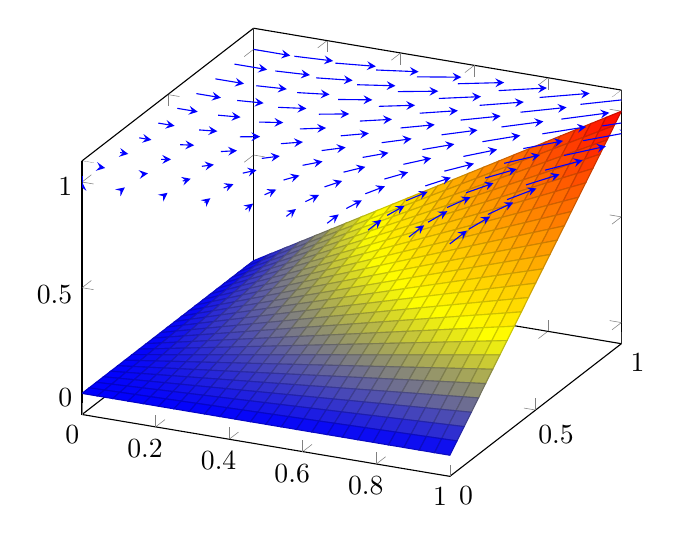
\begin{tikzpicture}
\begin{axis}[
    domain=0:1,
    xmax=1,
    ymax=1,
]
    \addplot3 [surf] {x*y};
    \addplot3 [
        blue,-stealth,samples=10,
        quiver,quiver/.cd,
            u=y,v=x,w=0,
            scale arrows=0.1,
    ] {1};
\end{axis}
\end{tikzpicture}
\end{codeexample}
    %
    \noindent Here, the quiver plots is placed on top of a |surf|. It
    visualizes the gradient (using a common scale factor of $1/10$ to reduce
    the arrow lengths). The |quiver/w=0| means that arrows have no $z$
    difference, and the |{1}| argument indicates that all start at
    $(x_i,y_j,1)$. Here, the values $(x_i,y_j)$ are sampled in the |domain=0:1|
    argument (with |samples=10|), i.e.\@ arrows start at $(x_i,y_j,1)$ and end
    at $(x_i+y_j/10, y_j+x_i/10, 1)$.

    So far, quiver plots do not assume a special sequence of input points. This
    has two consequences: first, you can plot any vector field by considering
    just $(x,y) + (u,v)$ (or $(x,y,z) + (u,v,w)$) -- the data doesn't
    necessarily need to be a two-dimensional function (as opposed to |surf|
    etc). On the other hand, you need to provide |quiver/scale arrows| manually
    since |quiver| doesn't know the mesh width in case you provide matrix
    data\footnote{Actually, I might add something like \texttt{quiver/scale
    arrows=auto} in the future, I don't know yet. Loops through input data are
    slow in \TeX{}, automatic mesh widths computation even more\ldots}.

    Note that quiver plots are currently not available together with
    logarithmic axes.

    \begin{pgfplotskeylist}{%
        quiver/u=\meta{expression} (initially 0),
        quiver/v=\meta{expression} (initially 0),
        quiver/w=\meta{expression} (initially 0)%
    }
        These keys define how the vector directions $(u,v)$ (or, for three
        dimensional plots, $(u,v,w)$) shall be set.

        The \meta{expression} can be a constant expression like |quiver/u=1| or
        |quiver/u=42*5|. It may also depend on the final base point values
        using the values |x|, |y| or |z| as in the example above. In this
        context, |x| yields the $x$-coordinate of the point where the vector
        starts, |y| the $y$-coordinate and so on.


        \paragraph{Attention:}

        the fact that |x| refers to \emph{the final $x$-coordinate} means that
        parametric plots \emph{should use $t$ as variable}\footnote{Sorry for
        this usability issue.}. Consider the following example:
        %
\begin{codeexample}[]
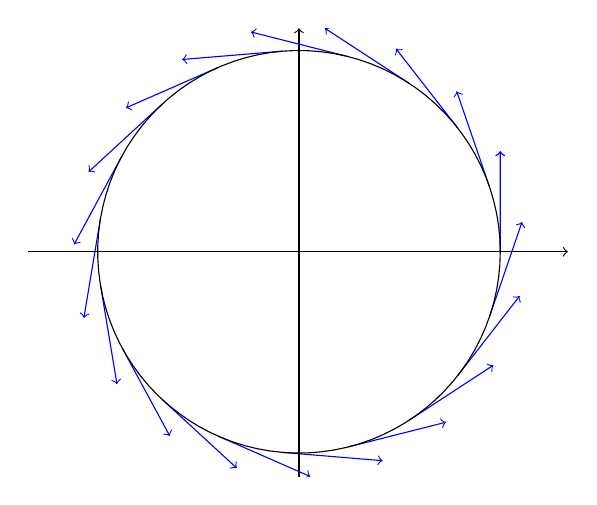
\begin{tikzpicture}
\begin{axis}[
    axis equal,
    axis lines=middle,
    axis line style={->},
    tick style={color=black},
    xtick=\empty,ytick=\empty,
]
    \addplot [samples=20, domain=0:2*pi,->,blue,
        % the default choice 'variable=\x' leads to
        % unexpected results here!
        variable=\t,
        quiver={
            u={-sin(deg(t))},
            v={cos(deg(t))},
            scale arrows=0.5,
        },
    ] ( {cos(deg(t))}, {sin(deg(t))} );
    \addplot [
        samples=100, domain=0:2*pi,
    ] ( {cos(deg(x))}, {sin(deg(x))} );
\end{axis}
\end{tikzpicture}
\end{codeexample}
        %
        \noindent Here, a parametric plot is used to draw a circle and tangent
        vectors. The choice |variable=\t| plays a functional role besides
        naming conventions: it allows to access the parametric variable within
        the expressions for both |u| and |v|. On the other hand, we could have
        used |u=y| and |v=-x| since |x| expands to the $x$~coordinate with
        value |sin(deg(t))| and |y| expands to the $y$~coordinate
        |cos(deg(t))|.

        Another important application is to use \emph{table column references}
        like |quiver/u=\thisrow{col}| in conjunction with |\addplot table|:
        %
\begin{codeexample}[]
\begin{tikzpicture}
\begin{axis}[title=Quiver and plot table]
    \addplot [
        blue,
        quiver={u=\thisrow{u},v=\thisrow{v}},
        -stealth,
    ] table {
        x y u v
        0 0 1 0
        1 1 1 1
        2 4 1 4
        3 9 1 6
        4 16 1 8
    };
\end{axis}
\end{tikzpicture}
\end{codeexample}
        %
        \noindent Here, the \meta{expression} employs |\thisrow| which always
        refers to the actual row of |\addplot table|.

        Note that \meta{expression} should always be of numeric type (no
        symbolic input extensions are supported currently).
    \end{pgfplotskeylist}

    \begin{pgfplotskeylist}{%
        quiver/u value=\marg{value} (initially 0),
        quiver/v value=\marg{value} (initially 0),
        quiver/w value=\marg{value} (initially 0)%
    }
        These keys have the \emph{same function} as |quiver/u| and its
        variants. However, they don't call the math parser, so only single
        values are allowed (including something like |\thisrow{columnname}|).
    \end{pgfplotskeylist}

    \begin{pgfplotskeylist}{%
        quiver/colored,
        quiver/colored=\marg{color}%
    }
        Allows to define an individual color for each arrow. Omitting the
        argument `\meta{color}' is identical to |quiver/colored=mapped color|
        which uses the |point meta| to get colors for every arrow.

        If you just want to set the same color for every arrow, prefer using
        |\addplot[blue,quiver]| which is more efficient.
    \end{pgfplotskeylist}

    \begin{pgfplotskey}{quiver/scale arrows=\marg{scale} (initially 1)}
        Allows to rescale the arrows by a factor. This may be necessary if the
        arrow length is longer than the distance between adjacent base points
        $(x_i,y_i)$. There may come a feature to rescale them automatically.
    \end{pgfplotskey}

    \begin{pgfplotskey}{quiver/update limits=\mchoice{true,false} (initially true)}
        A boolean indicating whether points $(x,y) + (u,v)$ shall contribute
        to the axis limits.
    \end{pgfplotskey}

    \begin{stylekey}{/pgfplots/quiver/every arrow (initially empty)}
        Allows to provide individual arrow styles.

        The style can contain any \Tikz{} drawing option. It will be evaluated
        for every individual arrow and may depend upon anything which is
        available at visualization time.

        In particular, this includes |point meta| data, typically using
        |\pgfplotspointmetatransformed| $\in [0,1000]$ where~$0$ corresponds to
        |point meta min| and~$1000$ corresponds to |point meta max|:
        %
    \label{pgfplots:example:pointmeta:quiver}
\begin{codeexample}[]
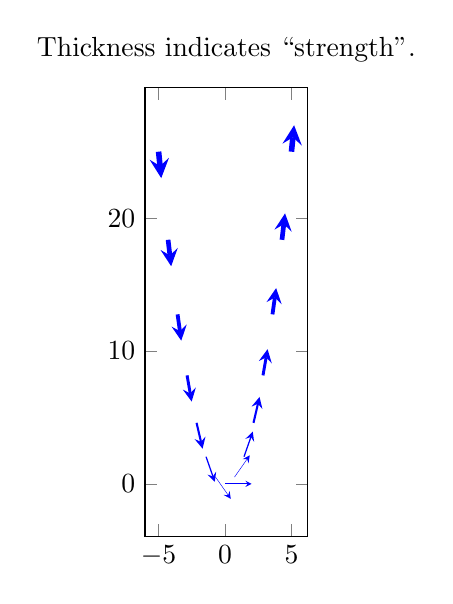
\begin{tikzpicture}
% define some constants:
\def\U{1}
\def\V{2*x}
\def\LEN{(sqrt((\U)^2 + (\V)^2)}

\begin{axis}[axis equal image,
    title=Thickness indicates ``strength''.
]
\addplot [blue,
  point meta={\LEN},
  quiver={
   u={(\U)/\LEN}, v={(\V)/\LEN},
   scale arrows=2,
   every arrow/.append style={
    line width=2pt*\pgfplotspointmetatransformed/1000
   },
  },
  -stealth,samples=15,
] {x^2};
\end{axis}
\end{tikzpicture}
\end{codeexample}
        %
        \noindent In the example, we have some 2d vector field stored in helper
        constants |\U| and |\V|. The length of each vector is stored in |\LEN|
        here. The |quiver| plot as such contains unit length vectors -- and the
        |\LEN| enters an |every arrow| style to get varying |line width|.

        An |every arrow| style might also depend upon |mapped color| (provided
        |point meta| has been set).

        Again, if you do not need individual arrow styles, prefer using a plot
        style (|cycle list| or argument to |\addplot|) which is more efficient.
    \end{stylekey}

    \begin{pgfplotsxycodekeylist}{
        quiver/before arrow,
        quiver/after arrow%
    }
        Advanced keys for more fine tuning of the display. They allow to
        install some \TeX{} code manually before or after the drawing
        operations for single arrows. Both are initially empty.
    \end{pgfplotsxycodekeylist}

    \begin{stylekey}{/pgfplots/quiver/quiver legend}
        A style which redefines |legend image code| in order to produce a
        suitable legend for |quiver| plots.

        It is implicitly activated whenever |quiver| plot handlers are
        selected.
        %
\begin{codeexample}[]
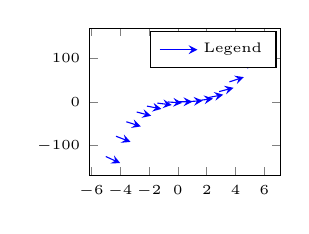
\begin{tikzpicture}
\begin{axis}[tiny]
    \addplot [
        blue,
        quiver={u=1,v=3*x},
        -stealth,
        samples=15,
    ] {x^3};
        \addlegendentry{Legend}
\end{axis}
\end{tikzpicture}
\end{codeexample}
    \end{stylekey}
\end{plottype}


\subsection{Stacked Plots}

\begin{pgfplotskey}{stack plots=\mchoice{x,y,false} (initially false)}
    Allows stacking of plots in either $x$ or $y$ direction. Stacking means to
    add either $x$- or $y$-coordinates of successive |\addplot| commands on top
    of each other.
    %
\begin{codeexample}[]
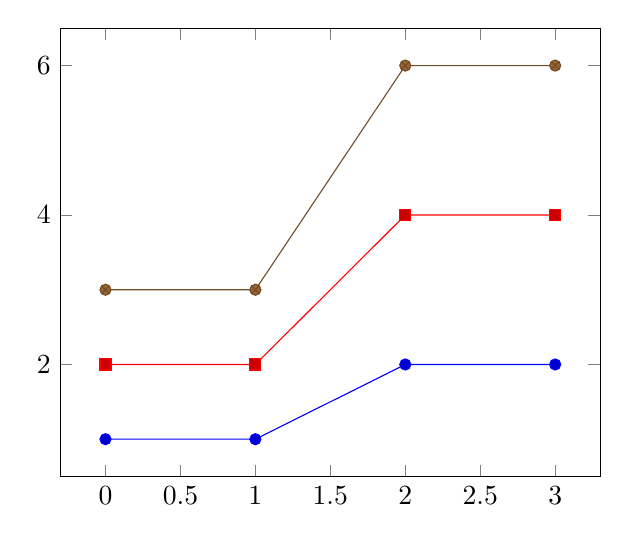
\begin{tikzpicture}
\begin{axis}[stack plots=y]
    \addplot coordinates {
        (0,1) (1,1) (2,2) (3,2)
    };
    \addplot coordinates {
        (0,1) (1,1) (2,2) (3,2)
    };
    \addplot coordinates {
        (0,1) (1,1) (2,2) (3,2)
    };
\end{axis}
\end{tikzpicture}
\end{codeexample}
    %
    The current implementation for |stack plots| does \emph{not} interpolate
    missing coordinates. That means stacking will fail if the plots have
    different grids.
\end{pgfplotskey}

\begin{stylekey}{/pgfplots/ybar stacked=\mchoice{plus,minus} (default plus)}
    The plot handler |stack plots| is particularly useful for bar plots. There
    are two possible modes of operation: the first is to set
    |stack plots=y,/tikz/ybar|. It activates just these two features without
    making them aware of each other. The second is to set |ybar stacked| which
    activates the two features \emph{and} makes them aware of each other.

    If you use |stack plots| together with |/tikz/ybar|, you have kind of a
    low-level implementation which is kind of ``raw'':

\begin{codeexample}[]
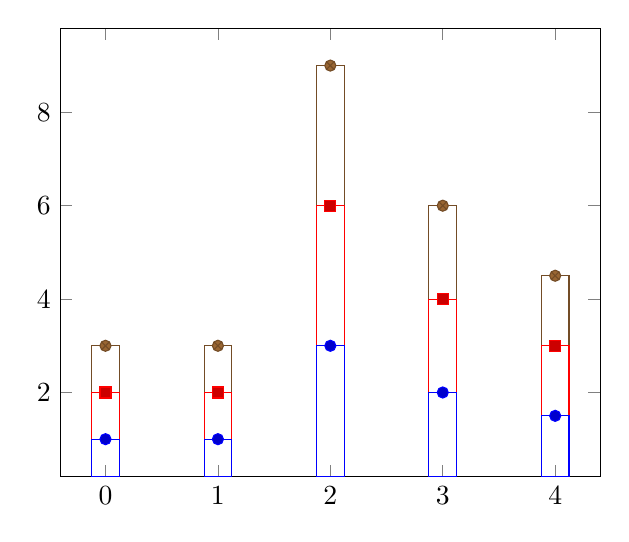
\begin{tikzpicture}
\begin{axis}[stack plots=y,/tikz/ybar]
    \addplot coordinates {
        (0,1) (1,1) (2,3) (3,2) (4,1.5)
    };
    \addplot coordinates {
        (0,1) (1,1) (2,3) (3,2) (4,1.5)
    };
    \addplot coordinates {
        (0,1) (1,1) (2,3) (3,2) (4,1.5)
    };
\end{axis}
\end{tikzpicture}
\end{codeexample}

    Using |ybar stacked| enables stacked vertical bars (i.e.\@ |ybar| and
    |stack plots=y|) \emph{and} it also adjusts the legend and tick appearance
    and assigns a useful |cycle list|. To this end, it should be given as
    option to the axis:
    %
\begin{codeexample}[]
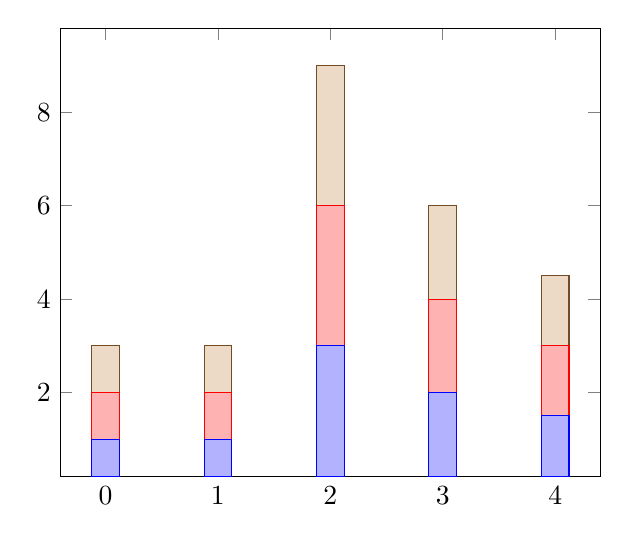
\begin{tikzpicture}
\begin{axis}[ybar stacked]
    \addplot coordinates {
        (0,1) (1,1) (2,3) (3,2) (4,1.5)
    };
    \addplot coordinates {
        (0,1) (1,1) (2,3) (3,2) (4,1.5)
    };
    \addplot coordinates {
        (0,1) (1,1) (2,3) (3,2) (4,1.5)
    };
\end{axis}
\end{tikzpicture}
\end{codeexample}

\begin{codeexample}[]
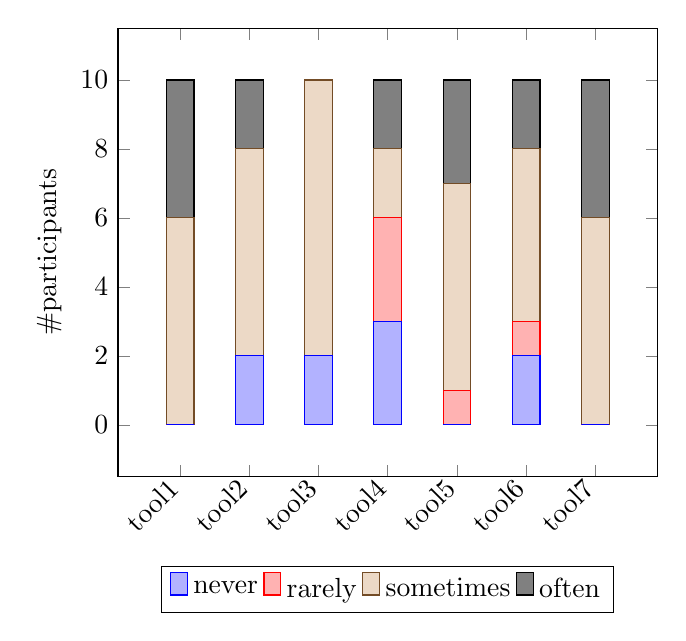
\begin{tikzpicture}
\begin{axis}[
    ybar stacked,
    enlargelimits=0.15,
    legend style={at={(0.5,-0.20)},
        anchor=north,legend columns=-1},
    ylabel={\#participants},
    symbolic x coords={tool1, tool2, tool3, tool4,
        tool5, tool6, tool7},
    xtick=data,
    x tick label style={rotate=45,anchor=east},
]
\addplot+ [ybar] coordinates {(tool1,0) (tool2,2)
  (tool3,2) (tool4,3) (tool5,0) (tool6,2) (tool7,0)};
\addplot+ [ybar] coordinates {(tool1,0) (tool2,0)
  (tool3,0) (tool4,3) (tool5,1) (tool6,1) (tool7,0)};
\addplot+ [ybar] coordinates {(tool1,6) (tool2,6)
  (tool3,8) (tool4,2) (tool5,6) (tool6,5) (tool7,6)};
\addplot+ [ybar] coordinates {(tool1,4) (tool2,2)
  (tool3,0) (tool4,2) (tool5,3) (tool6,2) (tool7,4)};
\legend{never, rarely, sometimes, often}
\end{axis}
\end{tikzpicture}
\end{codeexample}
\end{stylekey}

\begin{stylekey}{/pgfplots/xbar stacked=\mchoice{plus,minus} (default plus)}
    The same remarks as for |ybar stacked| hold for |xbar stacked| as well:
    |xbar stacked| is a figure-wide style which enables stacked horizontal bars
    (i.e.\@ |xbar| and |stack plots=x|). It also adjusts the legend and tick
    appearance and assigns a useful |cycle list|.

    Consequently, one can have a ``raw'' picture which combines stacking and
    bars as in the following picture (i.e.\@ without |xbar stacked|):
    %
\begin{codeexample}[]
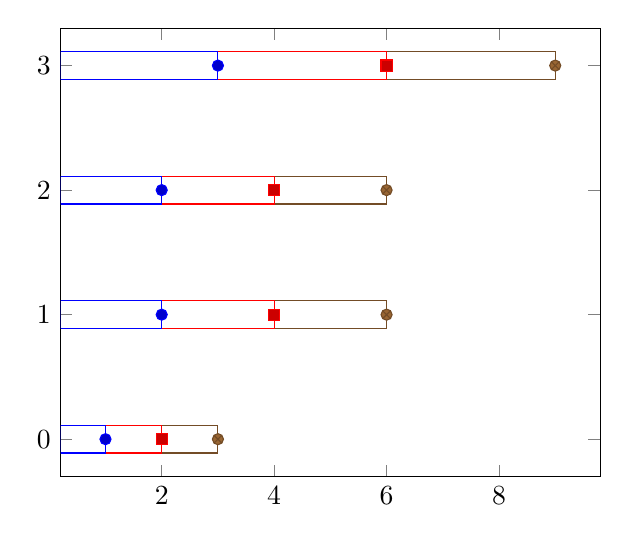
\begin{tikzpicture}
\begin{axis}[stack plots=x,/tikz/xbar]
    \addplot coordinates {
        (1,0) (2,1) (2,2) (3,3)
    };
    \addplot coordinates {
        (1,0) (2,1) (2,2) (3,3)
    };
    \addplot coordinates {
        (1,0) (2,1) (2,2) (3,3)
    };
\end{axis}
\end{tikzpicture}
\end{codeexample}

    Alternatively, one activates |xbar stacked| right after |\begin{axis}| and
    benefits from several style adoptions.
    %
\begin{codeexample}[]
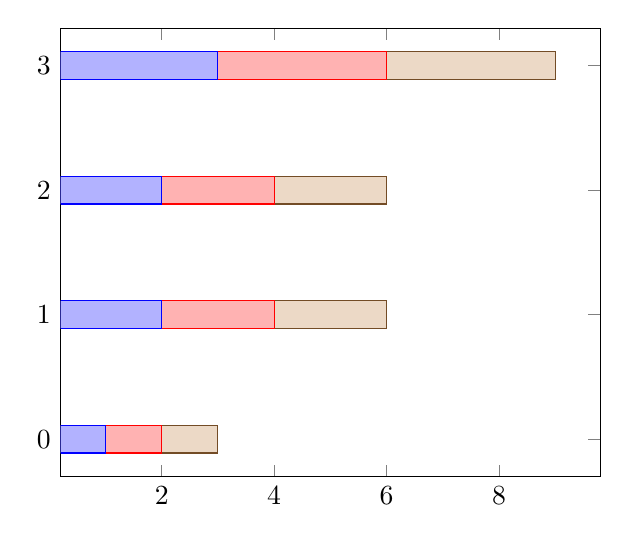
\begin{tikzpicture}
\begin{axis}[xbar stacked]
    \addplot coordinates {
        (1,0) (2,1) (2,2) (3,3)
    };
    \addplot coordinates {
        (1,0) (2,1) (2,2) (3,3)
    };
    \addplot coordinates {
        (1,0) (2,1) (2,2) (3,3)
    };
\end{axis}
\end{tikzpicture}
\end{codeexample}
\end{stylekey}

\begin{pgfplotskey}{stack dir=\mchoice{plus,minus} (initially plus)}
    Configures the direction of |stack plots|. The value |plus| will add
    coordinates of successive plots while |minus| subtracts them.
\end{pgfplotskey}

\begin{pgfplotskey}{reverse stacked plots=\mchoice{true,false} (initially true, default true)}
    Configures the sequence in which stacked plots are drawn. This is more or
    less a technical detail which should not be changed in any normal case.

    The motivation is as follows: suppose multiple |\addplot| commands are
    stacked on top of each other and they are processed in the order of
    appearance. Then, the second plot could easily draw its lines (or fill
    area) on top of the first one -- hiding its marker or line completely.
    Therefor, \PGFPlots{} reverses the sequence of drawing commands.

    This has the side-effect that any normal \Tikz{} paths inside of an axis
    will also be processed in reverse sequence.
\end{pgfplotskey}

\begin{pgfplotskey}{stacked ignores zero=\mchoice{true,false} (initially true, default true)}
    Configures stacked plots to ignore ``zero'' increments.

    In this context, ``ignore'' means to suppress visualization if an increment
    vanishes.

    Configuring |\pgfplotsset{compat=1.9}| (or higher) activates this feature
    for |xbar stacked| and |ybar stacked|.

    \begin{pgfplotskeylist}{%
        stacked ignores zero/default=\mchoice{true,false} (initially true),
        stacked ignores zero/markers=\mchoice{true,false} (initially true),
        stacked ignores zero/errorbars=\mchoice{true,false} (initially false)%
    }
        A detail key which allows to customize how and where to apply
        |stacked ignores zero|. This key is \emph{ignored} unless
        |stacked ignores zero=true|. Its default configuration is to suppress
        visualization of an empty increment for the standard visualization and
        for markers. Error bars will be displayed, though (the error bar is
        typically non-empty even if the increment is $0$).
    \end{pgfplotskeylist}
\end{pgfplotskey}

\begin{stylekey}{/pgfplots/xbar interval stacked=\mchoice{plus,minus} (default plus)}
    A style similar to |/pgfplots/xbar stacked| for the interval based bar plot
    variant.
\end{stylekey}

\begin{stylekey}{/pgfplots/ybar interval stacked=\mchoice{plus,minus} (default plus)}
    A style similar to |/pgfplots/ybar stacked| for the interval based bar plot
    variant.
\end{stylekey}


\subsubsection{Stacked Bar Plots and Nodes Near Coords}

It is possible to combine |ybar stacked| and |xbar stacked| with
|nodes near coords|. In contrast to non-stacked plots, it appears to be of
limited use to draw a node near the top of the stack. Instead, one typically
wants to see the \emph{difference} added in each stacking step. To this end,
\PGFPlots{} will automatically reconfigure |nodes near coords| to display the
added values in the center of each new bar:

\begin{codeexample}[]
% needs \pgfplotsset{compat=1.9} or newer!
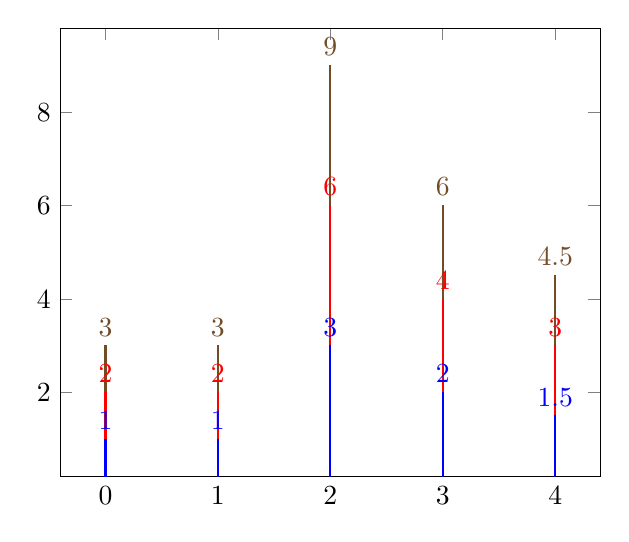
\begin{tikzpicture}
\begin{axis}[
    ybar stacked,nodes near coords,
    bar width=0.4,
]
    \addplot coordinates
        {(0,1) (1,1) (2,3) (3,2) (4,1.5)};
    \addplot coordinates
        {(0,1) (1,1) (2,3) (3,2) (4,1.5)};
    \addplot coordinates
        {(0,1) (1,1) (2,3) (3,2) (4,1.5)};
\end{axis}
\end{tikzpicture}
\end{codeexample}

\begin{codeexample}[]
% needs \pgfplotsset{compat=1.9} or newer!
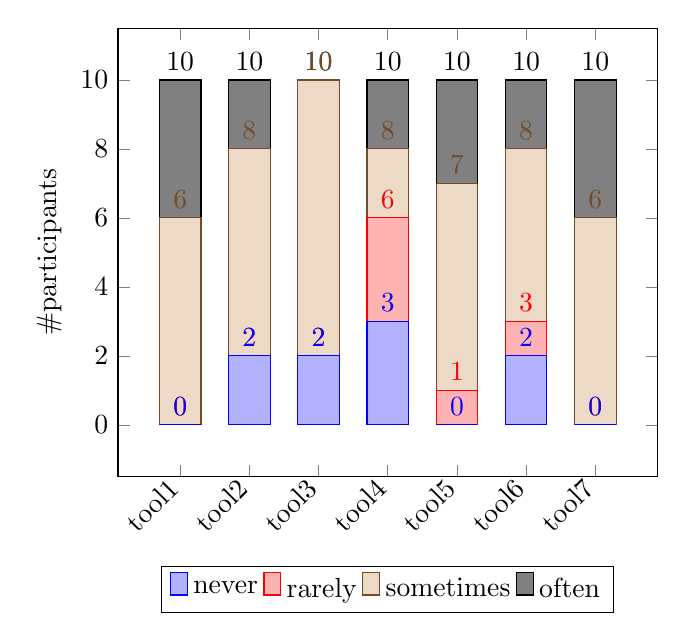
\begin{tikzpicture}
\begin{axis}[
    ybar stacked,
    bar width=15pt,
    nodes near coords,
    enlargelimits=0.15,
    legend style={at={(0.5,-0.20)},
        anchor=north,legend columns=-1},
    ylabel={\#participants},
    symbolic x coords={tool1, tool2, tool3, tool4,
        tool5, tool6, tool7},
    xtick=data,
    x tick label style={rotate=45,anchor=east},
]
\addplot+ [ybar] coordinates {(tool1,0) (tool2,2)
  (tool3,2) (tool4,3) (tool5,0) (tool6,2) (tool7,0)};
\addplot+ [ybar] coordinates {(tool1,0) (tool2,0)
  (tool3,0) (tool4,3) (tool5,1) (tool6,1) (tool7,0)};
\addplot+ [ybar] coordinates {(tool1,6) (tool2,6)
  (tool3,8) (tool4,2) (tool5,6) (tool6,5) (tool7,6)};
\addplot+ [ybar] coordinates {(tool1,4) (tool2,2)
  (tool3,0) (tool4,2) (tool5,3) (tool6,2) (tool7,4)};
\legend{never, rarely, sometimes, often}
\end{axis}
\end{tikzpicture}
\end{codeexample}

Note that the preceding example contains no nodes for coordinates with
value~|0|. This is due to the key |stacked ignores zero| which is active if
|compat=1.9| or newer: empty increments will be discarded.

This automatic reconfiguration is essentially part of the styles |xbar stacked|
or |ybar stacked|: both reconfigure |nodes near coords|. Note that this
feature has been introduced in version 1.9. In order to maintain backwards
compatible to previous workarounds, you have to write |compat=1.9| to get these
effects.

\begin{codeexample}[]
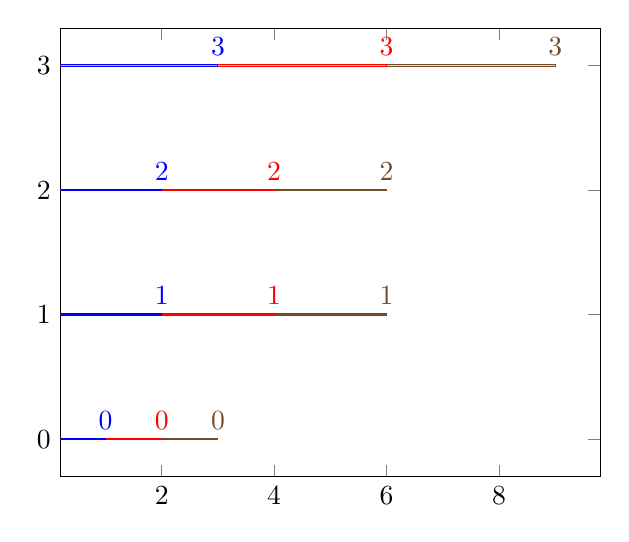
\begin{tikzpicture}
\begin{axis}[
    xbar stacked,nodes near coords,
    bar width=0.5,
]
    \addplot coordinates
        {(1,0) (2,1) (2,2) (3,3)};
    \addplot coordinates
        {(1,0) (2,1) (2,2) (3,3)};
    \addplot coordinates
        {(1,0) (2,1) (2,2) (3,3)};
\end{axis}
\end{tikzpicture}
\end{codeexample}


\subsubsection{Stacked Plots with Negative Values}

The meaning of negative values in |xbar stacked| or |ybar stacked| and their
visualization depends on the use case, and they need to be defined. \PGFPlots{}
offers two different interpretations of negative values in the context of
stacked plots:

\begin{pgfplotskey}{stack negative=\mchoice{on previous,separate} (initially separate)}
    The choice \declaretext{on previous} will simply sum any values as they are
    found in the input data. Thus, if you have four plots which are stacked on
    top of each other, and the first has value $10$, the second value $50$, and
    the third value $-10$, and the fourth has $30$, the final value will be
    $10+50-10+30 = 80$. However, visualizing a bar of negative size as a usual
    |xbar stacked| graph is hard to read and requires vertical offsets in this
    context. This can be accomplished as follows:
    %
\begin{codeexample}[]
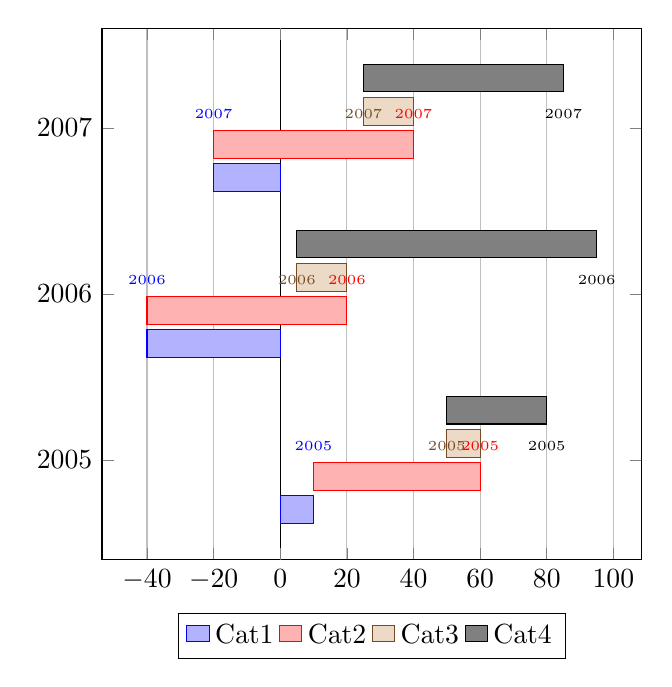
\begin{tikzpicture}
    \pgfplotstableread{
        Year  Cat1  Cat2  Cat3  Cat4
        2005  10    50    -10   30
        2006  -40   60    -15   90
        2007  -20   60    -15   60
    }\mytable
\begin{axis}[
    xbar stacked,
    stack negative=on previous,
    %
    xmajorgrids,
    legend style={at={(0.5,-0.1)},
        anchor=north,legend columns=-1},
    bar width=10pt,
    bar shift auto,
    nodes near coords,
    nodes near coords style={font=\tiny},
    y=60pt,
    ytick distance=1,
    enlarge y limits=0.3,
    /pgf/number format/1000 sep=,
    extra x ticks={0},
    extra x tick style={grid style={black},
    xticklabel=\empty},
]
    \addplot table [x index=1,y=Year] {\mytable};
    \addplot table [x index=2,y=Year] {\mytable};
    \addplot table [x index=3,y=Year] {\mytable};
    \addplot table [x index=4,y=Year] {\mytable};
    \legend{Cat1,Cat2,Cat3,Cat4}
\end{axis}
\end{tikzpicture}
\end{codeexample}

    In this case, the values for $y=2005$ resemble our input case of
    $10+50-10+30=80$. It is a ``normal'' |xbar stacked| with the configuration
    |stack negative=on previous| -- but with the special key |bar shift auto|
    which is also used in order to create grouped |xbar| charts: every
    |\addplot| receives a vertical offset.

    Despite the similarity with ``waterfall charts''\index{waterfall chart},
    this is not indented to be a waterfall chart. At the time of this writing,
    \PGFPlots{} has no support for waterfall charts.

    The choice |stack negative=on previous| is the \emph{initial} value for
    %
    \begin{itemize}
        \item all but stacked bar plots,
        \item all plots if |compat| is less than |1.13|.
    \end{itemize}
    %
    As of |compat=1.13|, the initial value of |stack negative| is |separate|
    for |xbar stacked|, |ybar stacked|, and their |* interval| based variants.

    The alternative choice \declaretext{separate} tracks the start points of
    bars \emph{separately} for negative and non-negative values:
    %
\begin{codeexample}[]
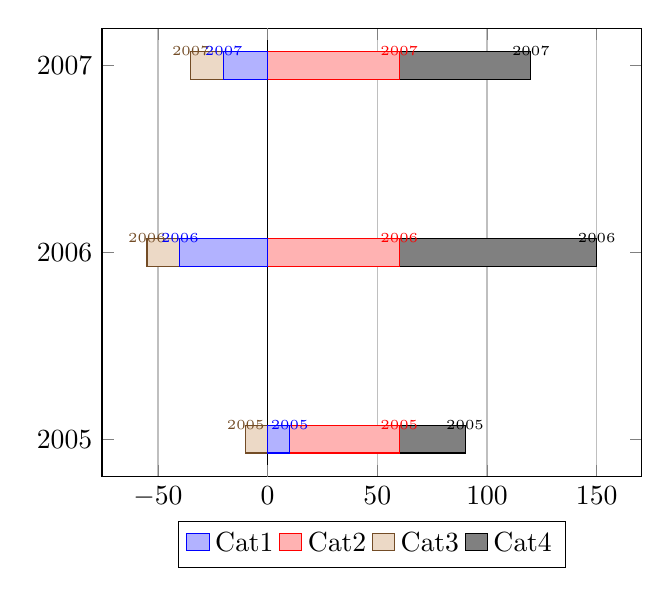
\begin{tikzpicture}
    \pgfplotstableread{
        Year  Cat1  Cat2  Cat3  Cat4
        2005  10    50    -10   30
        2006  -40   60    -15   90
        2007  -20   60    -15   60
    }\mytable
\begin{axis}[
    xbar stacked,
    % is default anyway:
    stack negative=separate,
    %
    /pgf/number format/1000 sep=,
    xmajorgrids,
    nodes near coords,
    nodes near coords style={font=\tiny},
    ytick distance=1,
    legend style={at={(0.5,-0.1)},
        anchor=north,legend columns=-1},
    extra x ticks={0},
    extra x tick style={grid style={black},
    xticklabel=\empty},
]
    \addplot table [x index=1,y=Year] {\mytable};
    \addplot table [x index=2,y=Year] {\mytable};
    \addplot table [x index=3,y=Year] {\mytable};
    \addplot table [x index=4,y=Year] {\mytable};
    \legend{Cat1,Cat2,Cat3,Cat4}
\end{axis}
\end{tikzpicture}
\end{codeexample}

    In this case, positive contributions extend into the positive $x$-axis
    whereas negative contributions extend into the negative $x$-axis. There is
    no final sum (or better: there are two final sums). The effect is as if you
    would have defined two separate axes, one for the positive contributions
    and one for the negative ones and aligned them at the origin.

    As of |compat=1.13|, |stack negative=separate| is the initial setting for
    stacked bar plots. Older compatibility levels use
    |stack negative=on previous|.
\end{pgfplotskey}


\subsection{Area Plots}

Area plots means two-dimensional plots in which an area is filled between a
couple of curves. Note that this is a rather incomplete characterization as
|mesh|, |surf|ace, and |patch| plots are, of course, also ``area plots'' of
some sort.

This section covers two types of area plots, namely those which are defined by
|stack plots| and those which are defined using |\addplot fill between|.


\subsubsection{Filling Using Stacked Plots}

The first (and older) option to fill areas between plots is a combination of
|\closedcycle| and |stack plots|. They can be combined with any other plot
type.

\begin{codeexample}[]
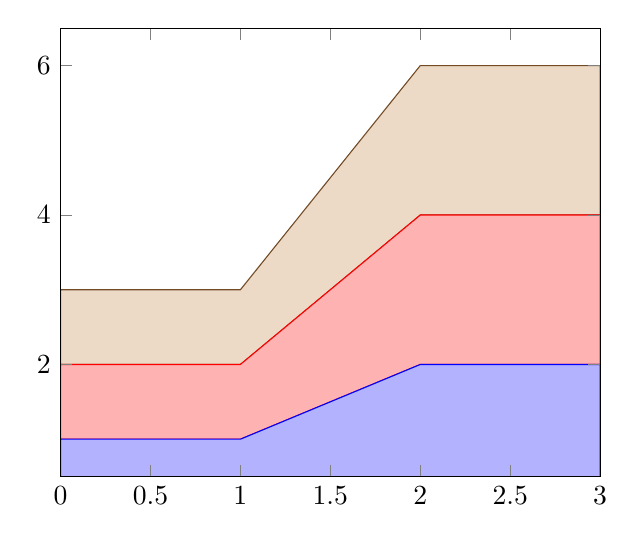
\begin{tikzpicture}
\begin{axis}[
    stack plots=y,
    area style,
    enlarge x limits=false,
]
    \addplot coordinates
        {(0,1) (1,1) (2,2) (3,2)}
            \closedcycle;
    \addplot coordinates
        {(0,1) (1,1) (2,2) (3,2)}
            \closedcycle;
    \addplot coordinates
        {(0,1) (1,1) (2,2) (3,2)}
            \closedcycle;
    \end{axis}
\end{tikzpicture}
\end{codeexample}
%
\noindent The main property of this kind of area visualization is that all
plots of an axis are taken together, and since they are stacked, they form
areas.

\noindent Area plots may need modified legends, for example using the
|area legend| key. Furthermore, one may want to consider the |axis on top| key
such that filled areas do not overlap ticks and grid lines since such plots
typically cover huge areas of the axis.

Note that Area plots which rely on |stack plots| have one severe limitation:
stacking works if and only if each plot has the same coordinates (in our case
of |stack plots=y|, each plot has the same $x$~coordinates).

\begin{stylekey}{/pgfplots/area style}
    A style which sets
    %
\begin{codeexample}[code only]
\pgfplotsset{
    /pgfplots/area style/.style={
        area cycle list,
        area legend,
        axis on top,
    },
}
\end{codeexample}
\end{stylekey}

\begin{stylekey}{/pgfplots/area cycle list}
    A style which installs a |cycle list| suitable for area plots. The initial
    configuration of this style simply invokes the |bar cycle list| which does
    also provide filled plot styles.
\end{stylekey}

\begin{codeexample}[]
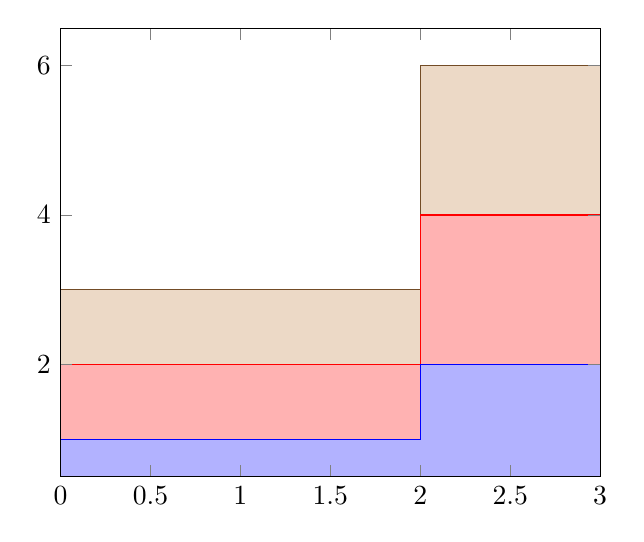
\begin{tikzpicture}
    \begin{axis}[
        const plot,
        stack plots=y,
        area style,
        enlarge x limits=false,
    ]
    \addplot coordinates
        {(0,1) (1,1) (2,2) (3,2)}
            \closedcycle;
    \addplot coordinates
        {(0,1) (1,1) (2,2) (3,2)}
            \closedcycle;
    \addplot coordinates
        {(0,1) (1,1) (2,2) (3,2)}
            \closedcycle;
    \end{axis}
\end{tikzpicture}
\end{codeexample}

\begin{codeexample}[]
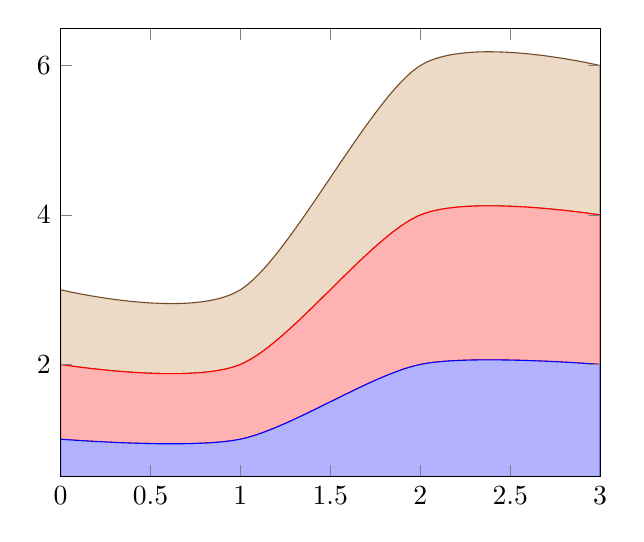
\begin{tikzpicture}
    \begin{axis}[
        smooth,
        stack plots=y,
        area style,
        enlarge x limits=false,
    ]
    \addplot coordinates
        {(0,1) (1,1) (2,2) (3,2)}
            \closedcycle;
    \addplot coordinates
        {(0,1) (1,1) (2,2) (3,2)}
            \closedcycle;
    \addplot coordinates
        {(0,1) (1,1) (2,2) (3,2)}
            \closedcycle;
    \end{axis}
\end{tikzpicture}
\end{codeexample}

\begin{codeexample}[]
\pgfplotstableread{pgfplots.timeseries.dat}\loadedtable
\pgfplotstabletypeset\loadedtable
\end{codeexample}

\begin{codeexample}[]
    \pgfplotstableread{pgfplots.timeseries.dat}{\loadedtable}
\begin{tikzpicture}
    \begin{axis}[
        ymin=0,
        minor tick num=4,
        enlarge x limits=false,
        axis on top,
        every axis plot post/.append style={mark=none},
        const plot,
        legend style={
            area legend,
            at={(0.5,-0.15)},
            anchor=north,
            legend columns=-1,
        },
    ]
        \addplot [draw=blue,fill=blue!30!white]
            table [x=time,y=1minload]       from \loadedtable
                \closedcycle;
        \addplot table [x=time,y=nodes]     from \loadedtable;
        \addplot table [x=time,y=cpus]      from \loadedtable;
        \addplot table [x=time,y=processes] from \loadedtable;
        \legend{1min load,nodes,cpus,processes}
    \end{axis}
\end{tikzpicture}
\end{codeexample}

\begin{codeexample}[width=4cm]
    \pgfplotstableread{pgfplots.timeseries.dat}\loadedtable
\begin{tikzpicture}
    \begin{axis}[
        ymin=0,
        minor tick num=4,
        enlarge x limits=false,
        const plot,
        axis on top,
        stack plots=y,
        cycle list={
            {blue!70!black,fill=blue},
            {blue!60!white,fill=blue!30!white},
            {draw=none,fill={rgb:red,138;green,82;blue,232}},
            {red,thick}
        },
        ylabel={Mem [GB]},
        legend style={
            area legend,
            at={(0.5,-0.15)},
            anchor=north,
            legend columns=2},
    ]
    \addplot  table [x=time,y=memused]      from \loadedtable \closedcycle;
    \addplot  table [x=time,y=memcached]    from \loadedtable \closedcycle;
    \addplot  table [x=time,y=membuf]       from \loadedtable \closedcycle;
    \addplot+ [stack plots=false]
              table [x=time,y=memtotal]     from \loadedtable;
    \legend{Memory used,Memory cached,Memory buffered,Total memory}
    \end{axis}
\end{tikzpicture}
\end{codeexample}


\subsubsection{Filling Under/Between Named Plots}
\label{sec:fillbetween:in:area:plots}

{%
\pgfkeys{
    /pgfmanual/gray key prefixes/.add={}{,/tikz/fill between/},
    /pdflinks/search key prefixes in/.add={}{,/tikz/fill between/},
}

The second way to fill areas under or between plots is the |fillbetween|
library shipped with \PGFPlots{}.

\tikzname{} allows to name a plot or a path using |name path|. The
|fillbetween| library offers the special ``plot type'' |\addplot fill between|
which expects two such named paths on input. Then, it generates filled areas
between these named paths.

The biggest difference to Area plots by means of |stack plots| as discussed in
the previous section is that |\addplot fill between| accepts \emph{arbitrary}
input plots: the coordinates can vary, the ranges can vary, even |smooth| and
|sharp plot| can be combined. In addition, |\addplot fill between| allows to
select only subregions between the two input paths by means of its |soft clip|
feature, and it accepts individually styled fill segments using its styles
|every even segment|, |every segment no| \meta{index}, etc.

The reference documentation is Section~\ref{sec:fillbetween}, but the following
examples attempt to cover basic use cases around ``fill between''. Please refer
to the reference documentation in Section~\ref{sec:fillbetween} for an in-depth
discussion of every involved key.

The following advanced example selects two partial areas using |soft clip| in
order to fill these areas:
%
\begin{codeexample}[]
% requires \usepgfplotslibrary{fillbetween}
\begin{tikzpicture}
\begin{axis}
    \addplot+ [name path=A,domain=0:5] {x^2};

    \path [name path=B]
        (\pgfkeysvalueof{/pgfplots/xmin},0) --
        (\pgfkeysvalueof{/pgfplots/xmax},0);

    \addplot [gray] fill between [
        of=A and B,soft clip={domain=3:4},
    ];
    \addplot [gray!30] fill between [
        of=A and B,soft clip={domain=2:3},
    ];
\end{axis}
\end{tikzpicture}
\end{codeexample}

The preceding example is characterized by two paths, each of which is named
using |name path|. The path named `|A|' is a plot of $x^2$. The other path
named `|B|' is actually nothing but the visible $x$-axis, the |\path|
instruction means that it is not drawn at all. Note that
|\pgfkeysvalueof{/pgfplots/xmin}| expands to the visible lower $x$-axis limit.
Finally, we see two |\addplot fill between| instructions, both with the
selection |of=A and B| and both with (different) values of |soft clip|. The
|soft clip| key restricts the filled segments to the bounding rectangle defined
by some path \meta{lower corner}| rectangle |\meta{upper corner} where the two
arguments are the lower and upper corner of an invisible rectangular bounding
box. In our case, this bounding box has been defined by some |domain|
restriction and the upper and lower axis limits. Only those parts of the filled
segment makes up the result of |\addplot fill between|.

This restriction to a specific interval (or better: rectangle) is also
available when stroking the involved paths `|A|' or `|B|': \PGFPlots{} comes
with |decoration=soft clip| which can be combined with |postaction| as follows.
%
\begin{codeexample}[]
% requires \usepgfplotslibrary{fillbetween}
\begin{tikzpicture}
\begin{axis}
    % define some common macro
    \def\clippath{
        (3,-1) rectangle (4,100)
    }
    \draw [help lines] \clippath;

    \addplot+ [name path=A,domain=0:5,
        mark=none,
        postaction={decorate,red,line width=2pt,
            decoration={
                soft clip,
                soft clip path={\clippath},
            },
        },
    ] {x^2};

    \path [name path=B]
        (\pgfkeysvalueof{/pgfplots/xmin},0) --
        (\pgfkeysvalueof{/pgfplots/xmax},0);

    \addplot [orange] fill between [
        of=A and B,soft clip={\clippath},
    ];
\end{axis}
\end{tikzpicture}
\end{codeexample}
%
The preceding example has a |\def\clippath| which defines a re-usable bounding
box. Here, the |fill between| statement is similar to the preceding example,
with the only difference that our macro is used as value. The main difference
is the |postaction| in plot `|A|'. A |postaction| is a \tikzname{} construct
which allows to draw the same path twice. The second time the plot is drawn
makes use of the option list after |postaction|. In our case, it is a
|decoration| which will be drawn in |red| with thick lines. The |decoration|
applies a |soft clip| path. In this context, |soft clip| is applied to one path
only, but the idea is the same: only the parts within the |soft clip| argument
are displayed.

Note that |fill between| is also possible for arbitrary plots, not just the
$x$-axis. In fact, one can combine any two plots.
%
\begin{codeexample}[]
% requires \usepgfplotslibrary{fillbetween}
\begin{tikzpicture}
\begin{axis}
    \addplot [blue,name path=A,domain=0:5] {x^2};
    \addplot [red,name path=B,smooth] table {
        x y
        0 10
        1 8
        2 6
        3 1
        4 5
    };
    \addplot [gray!50] fill between [
        of=A and B,
        soft clip={domain=3:4},
    ];
    \addplot [gray!10,draw=black] fill between [
        of=A and B,
        soft clip={domain=1:2.5},
    ];
\end{axis}
\end{tikzpicture}
\end{codeexample}
%
\noindent The preceding example has two plots with a different number of
samples, a different range, and a different input method. Nevertheless, the
area between these two plots can be filled just as in the previous examples,
including any intersections.

It is also possible to define individual styles for the filled segments. To
this end, one has to set the |split| key which activates separate output paths.
This enables the use of special styles which is shown in in the following
example. Here, we have two styles with explicitly numbered segment indices:
%
\begin{codeexample}[]
% requires \usepgfplotslibrary{fillbetween}
\begin{tikzpicture}
\begin{axis}
    \addplot [blue,name path=A,domain=0:5] {x^2};
    \addplot [red,name path=B,smooth] table {
        x y
        0 10
        1 8
        2 6
        3 1
        4 5
    };
    \addplot [gray] fill between [
        of=A and B,
        split,
        every segment no 0/.style=
            {pattern color=gray!50,
             pattern=north east lines},
        every segment no 1/.style=
            {pattern=north west lines},
    ];
\end{axis}
\end{tikzpicture}
\end{codeexample}
%
\noindent Note that the example has no |soft clip| argument. Consequently, it
fills between the start and end points of the involved paths. The |split|
argument combined with the styles yields individually drawn fill segments.

Further reading: see Section~\ref{sec:fillbetween}.
}


\subsection{Closing Plots (Filling the Area Under Plots)}
\label{sec:pgfplots:closingplots}

\begin{command}{\closedcycle}
    Provide |\closedcycle| as \meta{trailing path commands} after |\addplot| to
    draw a closed line from the last plot coordinate to the first one.

    Use |\closedcycle| whenever you intend to fill the area under a plot.

\begin{codeexample}[]
\begin{tikzpicture}
\begin{axis}
    \addplot {x^2+2} \closedcycle;
\end{axis}
\end{tikzpicture}
\end{codeexample}

\begin{codeexample}[]
\begin{tikzpicture}
\begin{axis}
    \addplot+ [fill] {x^2+2} \closedcycle;
\end{axis}
\end{tikzpicture}
\end{codeexample}
    %
    In case of stacked plots, |\closedcycle| connects the current plot with the
    previous plot instead of connecting with the $x$-axis.\footnote{The
    implementation for stacked plots requires some additional logic to
    determine the filled area: \lstinline{\\closedcycle} will produce a
    \texttt{plot coordinates} command with \emph{reversed} coordinates of the
    previous plot. This is usually irrelevant for end users, but it assumes
    that the plot's type is symmetric. Since constant plots are inherently
    asymmetric, \lstinline{\\closedcycle} will use \texttt{const plot mark
    right} as reversed sequence for \texttt{const plot mark left}.}
    %
\begin{codeexample}[]
\begin{tikzpicture}
\begin{axis}[stack plots=y]
    \addplot+ [fill] coordinates {
        (0,1) (1,1) (2,2) (3,2)
    }
        \closedcycle
    ;
    \addplot+ [fill] coordinates {
        (0,1) (1,1) (2,2) (3,2)
    }
        \closedcycle
    ;
\end{axis}
\end{tikzpicture}
\end{codeexample}
\end{command}

Closing a plot is also possible for \emph{three-dimensional axes}, see
Section~\ref{sec:pgfplots:filled:line} on
page~\pageref{sec:pgfplots:filled:line}.

Note that |\closedcycle| has been designed for functions (i.e.\@ for a plot
where every $x$ has at most one $y$ value). For arbitrary curves, you can
safely use the \tikzname{} path \declareandlabel{--cycle} instead which simply
connects the last and the first path element:
%
\begin{codeexample}[]
\begin{tikzpicture}
\begin{axis}
    \addplot coordinates {
        (0,1) (1,2) (0,3) (-1,2)
    };
\end{axis}
\end{tikzpicture}
\end{codeexample}

\begin{codeexample}[]
\begin{tikzpicture}
\begin{axis}
    \addplot coordinates {
        (0,1) (1,2) (0,3) (-1,2)
    }
        --cycle
    ;
\end{axis}
\end{tikzpicture}
\end{codeexample}

\begin{codeexample}[]
\begin{tikzpicture}
\begin{axis}
    \addplot+ [fill] coordinates {
        (0,1) (1,2) (0,3) (-1,2)
    }
        --cycle
    ;
\end{axis}
\end{tikzpicture}
\end{codeexample}

The |--cycle| is actually a path instruction of \cite{tikz}; it connects the
first and the last coordinate of one path. Note that this is automatically done
for |fill|ed paths.



\subsection{Scatter Plots}
\label{sec:pgfplots:scatter:2d}

The most simple scatter plots produce the same as the line plots above -- but
they contain only markers. They are enabled using the |only marks| key of
\Tikz{}.

\begin{plottype}{only marks}
    Draws a simple scatter plot: all markers have the same appearance.
    %
\begin{codeexample}[]
\begin{tikzpicture}
\begin{axis}[enlargelimits=false]
    \addplot+ [
        only marks,
        samples=400,
    ] {rand};
\end{axis}
\end{tikzpicture}
\end{codeexample}
    %
    The |only marks| visualization style simply draws marks at every
    coordinate. Marks can be set with |mark=|\meta{mark name} and marker
    options like size and color can be specified using the
    |mark options=|\meta{style options} key (or by modifying the |every mark|
    style). The available markers along with the accepted style options can be
    found in Section~\ref{sec:markers} on page~\pageref{sec:markers}.
\end{plottype}

    \label{pgfplots:scatter}
More sophisticated scatter plots change the marker appearance for each data
point. An example is that marker colors depend on the magnitude of function
values $f(x)$ or other provided coordinates. The term ``scatter plot'' will be
used for this type of plot in the following sections.

Scatter plots require ``source'' coordinates. These source coordinates can be
the $y$-coordinate, or explicitly provided additional values.

\begin{plottype}[/pgfplots]{scatter}
    Enables marker appearance modifications. The default implementation
    acquires ``source coordinates'' for every data point (see |scatter src|
    below) and maps them linearly into the current color map. The resulting
    color is used as draw and fill color of the marker.

\begin{codeexample}[]
\begin{tikzpicture}
\begin{axis}
    \addplot+ [
        scatter,
        only marks,
        samples=50,
        scatter src=y,
    ] {x - x^2};
\end{axis}
\end{tikzpicture}
\end{codeexample}

    The key |scatter| is simply a boolean variable which enables marker
    modifications. It applies only to markers and it can be combined with any
    other plot type.

\begin{codeexample}[]
\begin{tikzpicture}
\begin{axis}
    \addplot+ [
        scatter,
        samples=50,
        scatter src=y,
    ] {x^3};
\end{axis}
\end{tikzpicture}
\end{codeexample}
\end{plottype}

Scatter plots can be configured using a set of options. One of them is
mandatory, the rest allows fine grained control over marker appearance options.

\begin{pgfplotskey}{scatter src=\mchoice{%
        none,
        \meta{expression},
        x,y,z,
        f(x),
        explicit,
        explicit symbolic%
    } (initially none)%
}
\label{pgfplots:scatter:src}
    This key is necessary for any scatter plot and it is set to |f(x)| as soon
    as |scatter| is activated and no different choice has been made. It needs
    to be provided as \meta{option} for |\addplot| to configure the value used
    to determine marker appearances. Actually, |scatter src| is nothing but an
    alias for |point meta|, so the main documentation for this key is on
    page~\pageref{pgfplots:pointmeta}. However, we summarize the choices here
    together with scatter plot examples.

    Usually, |scatter src| provides input data (numeric or string type) which
    is used to determine colors and other style options for markers. The
    default configuration expects numerical data which is mapped linearly into
    the current color map.

    The value of |scatter src| determines how to get this data: the choices
    \declaretext{x}, \declaretext{y} and \declaretext{z} will use either the
    $x$-, $y$- or $z$-coordinates to determine marker options. Any coordinate
    filters, logarithms or stacked-plot computations have already been applied
    to these values (use |rawx|, |rawy| and |rawz| for unprocessed values). The
    special choice |f(x)| is the same as |y| for two dimensional plots and the
    same as |z| for three dimensional plots. The choice \declaretext{explicit}
    expects the scatter source data as additional coordinate from the
    coordinate input streams (see Section~\ref{pgfplots:providing:input} for
    how to provide input meta data or below for some small examples). They will
    be treated as numerical data. The choice \declaretext{explicit symbolic}
    also expects scatter source data as additional meta information for each
    input coordinate, but it treats them as strings, not as numerical data.
    Consequently, no arithmetics is performed. It is the task of the scatter
    plot style to do something with it. See, for example, the |scatter/classes|
    style below. Finally, it is possible to provide an arbitrary mathematical
    expression which involves zero, one or more of the values \declaretext{x}
    (the current $x$-coordinate), \declaretext{y} (the current $y$-coordinate)
    or \declaretext{z} (the current $z$-coordinate, if any).

    If data is read from tables, mathematical expressions might also involve
    |\thisrow|\marg{column name} or |\thisrowno|\marg{column index} to access
    any of the table cells in the current row.

    Here are examples for how to provide data for the choices
    \declaretext{explicit} and \declaretext{explicit symbolic}.
    %
\begin{codeexample}[code only]
\begin{tikzpicture}
    \begin{axis}
        % provide color data explicitly using [<data>]
        % behind coordinates:
        \addplot+ [scatter,scatter src=explicit]
            coordinates {
                (0,0) [1.0e10]
                (1,2) [1.1e10]
                (2,3) [1.2e10]
                (3,4) [1.3e10]
                % ...
            };

        % Assumes a datafile.dat like
        % xcolname  ycolname    colordata
        % 0         0           0.001
        % 1         2           0.3
        % 2         2.1         0.4
        % 3         3           0.5
        % ...
        % the file may have more columns.
        \addplot+ [scatter,scatter src=explicit]
            table [x=xcolname,y=ycolname,meta=colordata]
                {datafile.dat};
        % Same data as last example:
        \addplot+ [scatter,scatter src=\thisrow{colordata}+\thisrow{ycolname}]
            table [x=xcolname,y=ycolname]
                {datafile.dat};

        % Assumes a datafile.dat like
        % 0         0           0.001
        % 1         2           0.3
        % 2         2.1         0.4
        % 3         3           0.5
        % ...
        % the first three columns will be used here:
        \addplot+ [scatter,scatter src=explicit]
            file {datafile.dat};
    \end{axis}
\end{tikzpicture}
\end{codeexample}

    Please note that |scatter src|$\neq$|none| results in computational work
    even if |scatter=false|.
\end{pgfplotskey}

\begin{stylekey}{/pgfplots/scatter/use mapped color=\marg{options for each marker}
    (initially draw=mapped color!80!black,fill=mapped color)%
}
    This style is installed by default. When active, it recomputes the color
    |mapped color| for every processed point coordinate by transforming the
    |scatter src| coordinates into the current color map linearly. Then, it
    evaluates the options provided as \meta{options for each marker} which are
    expected to depend on |mapped color|.

    The user interface for color maps is described in
    Section~\ref{pgfplots:colormap}.

\begin{codeexample}[]
\begin{tikzpicture}
\begin{axis}[title=Default arguments]
    \addplot+ [
        scatter,
        scatter src=y,
    ] {2*x+3};
\end{axis}
\end{tikzpicture}
\end{codeexample}

\begin{codeexample}[]
\begin{tikzpicture}
\begin{axis}[
    title=Black fill color and varying draw color,
    scatter/use mapped color={
        draw=mapped color,
        fill=black,
    },
]
    \addplot+ [
        scatter,
        scatter src=y,
    ] {2*x+3};
\end{axis}
\end{tikzpicture}
\end{codeexample}

\begin{codeexample}[]
\begin{tikzpicture}
\begin{axis}[
    title=Black draw color and varying fill color,
    scatter/use mapped color={
        draw=black,
        fill=mapped color,
    },
]
    \addplot+ [
        scatter,
        scatter src=y,
    ] {2*x+3};
\end{axis}
\end{tikzpicture}
\end{codeexample}

\message{Expecting '/pgfplots/warning/approx empty range enlarged' here.^^J}%
\begin{codeexample}[]
\begin{tikzpicture}
    \begin{axis}[colormap/bluered,colorbar]
    \addplot3+ [
        samples=4,
        z buffer=sort,
        % enable scatter:
        scatter,
        % redefine appearance:
        scatter/use mapped color={ball color=mapped color},
        % configure input:
        scatter src=rand,
        only marks,
        mark=ball,
        mark size=3pt,
    ] {0};
    \end{axis}
\end{tikzpicture}
\end{codeexample}
    %
    This key is actually a style which redefines |@pre marker code| and
    |@post marker code| (see below).


    \paragraph{Remark:}

    The style |use mapped color| \emph{re}defines |@pre marker code| and
    |@post marker code|. There is a starred variant
    \declareandlabel{use mapped color*} which \emph{appends} the functionality
    while keeping the old marker code.
\end{stylekey}

\begin{stylekey}{/pgfplots/scatter/classes=\marg{styles for each class name}}
\label{pgfplots:scatterclasses}
    A scatter plot style which visualizes points using several classes. The
    style assumes that every point coordinate has a class label attached, that
    means the choice |scatter src=explicit symbolic| is assumed.\footnote{If
    \texttt{scatter src} is not \texttt{explicit symbolic}, we expect a numeric
    argument which is rounded to the nearest integer. The resulting integer is
    used as class label. If that fails, the numeric argument is truncated to
    the nearest integer. If that fails as well, the point has no label.} A
    class label can be a number, but it can also be a symbolic constant. Given
    class labels for every point, \meta{styles for each class name} contains a
    comma-separated list which associates appearance options to each class
    label.

\begin{codeexample}[]
\begin{tikzpicture}
\begin{axis}[
    scatter/classes={
        a={mark=square*,blue},
        b={mark=triangle*,red},
        c={mark=o,draw=black}   % <-- don't add comma
    },
]
    % \addplot[] is better than \addplot+[] here:
    % it avoids scalings of the cycle list
    \addplot [
        scatter,only marks,
        scatter src=explicit symbolic,
    ] coordinates {
        (0.1,0.15)  [a]
        (0.45,0.27) [c]
        (0.02,0.17) [a]
        (0.06,0.1)  [a]
        (0.9,0.5)   [b]
        (0.5,0.3)   [c]
        (0.85,0.52) [b]
        (0.12,0.05) [a]
        (0.73,0.45) [b]
        (0.53,0.25) [c]
        (0.76,0.5)  [b]
        (0.55,0.32) [c]
    };
\end{axis}
\end{tikzpicture}
\end{codeexample}
    %
    In this example, the coordinate |(0.1,0.15)| has the associated label `|a|'
    while |(0.45,0.27)| has the label `|c|' (see Section~\ref{sec:addplot} for
    details about specifying point meta data). Now, the argument to
    |scatter/classes| contains styles for every label -- for label `|a|',
    square markers will be drawn in color blue.

    The generation of a legend works as for a normal plot -- but
    |scatter/classes| requires one legend entry for every provided class. It
    communicates the class labels to the legend automatically. It works as if
    there had been different |\addplot| commands, one for every class label.

    It is also possible to provide |scatter/classes| as argument to a single
    plot, allowing different scatter plots in one axis.
    %
\begin{codeexample}[]
\begin{tikzpicture}
\begin{axis}[legend pos=south east]
    % The data file contains:
    % x     y      label
    % 0.1   0.15   a
    % 0.45  0.27   c
    % 0.02  0.17   a
    % 0.06  0.1    a
    % 0.9   0.5    b
    % 0.5   0.3    c
    % 0.85  0.52   b
    % 0.12  0.05   a
    % 0.73  0.45   b
    % 0.53  0.25   c
    % 0.76  0.5    b
    % 0.55  0.32   c
    \addplot [
        % clickable coords={\thisrow{label}},
        scatter/classes={
            a={mark=square*,blue},
            b={mark=triangle*,red},
            c={mark=o,draw=black,fill=black}% no comma
        },
        scatter,only marks,
        scatter src=explicit symbolic,
    ] table [x=x,y=y,meta=label]
        {plotdata/scattercl.dat};

    \addplot coordinates
        {(0.1,0.1) (0.5,0.3) (0.85,0.5)};
    \legend{Class 1,Class 2,Class 3,Line}
\end{axis}
\end{tikzpicture}
\end{codeexample}

    In general, the format of \meta{styles for each class name} is a comma
    separated list of \meta{label}|=|\marg{style options}.


    \paragraph{Attention:}

    The keys |every mark| and |mark options| have \emph{no effect} when used
    inside of \meta{styles for each class name}! So, instead of assigning
    |mark options|, you can simply provide the options directly. They apply only
    to markers anyway.


    \paragraph{Remark:}

    To use |\label| and |\ref| in conjunction with |scatter/classes|, you can
    provide the class labels as optional arguments to |\label| in square
    brackets:

\begin{codeexample}[code only]
\addplot [
    scatter/classes={
        a={mark=square*,blue},
        b={mark=triangle*,red},
        c={mark=o,draw=black,fill=black}    % <-- don't add comma here
    },
    scatter,only marks,
    scatter src=explicit symbolic,
]
    % [and coordinate input here... ]
;

\label[a]{label:for:first:class}
\label[b]{label:for:second:class}
\label[c]{label:for:third:class}

...
First class is \ref{label:for:first:class}, second is \ref{label:for:second:class}.
\end{codeexample}


    \paragraph{Remark:}

    It is possible to click into the plot to display labels with mouse popups,
    see the |clickable coords| key of the |clickable| library.

    \paragraph{Remark:}

    The style |scatter/classes| \emph{re}defines |@pre marker code| and
    |@post marker code|. There is a starred variant
    \declareandlabel{scatter/classes*} which \emph{appends} the functionality
    while keeping the old marker code.
\end{stylekey}

\begin{pgfplotskeylist}{%
    nodes near coords=\marg{content} (default \textbackslash pgfmathprintnumber\textbackslash pgfplotspointmeta),
    nodes near coords*=\marg{content} (default \textbackslash pgfmathprintnumber\textbackslash pgfplotspointmeta)%
}
    A |scatter| plot style which places text nodes near every coordinate.

\begin{codeexample}[]
\begin{tikzpicture}
\begin{axis}[nodes near coords]
    \addplot+ [
        only marks
    ] coordinates {
        (0.5,0.2) (0.2,0.1) (0.7,0.6)
        (0.35,0.4) (0.65,0.1)
    };
\end{axis}
\end{tikzpicture}
\end{codeexample}
    %
    The \meta{content} is, if nothing else has been specified, the content of
    the ``point meta'', displayed using the default
    \meta{content}=|\pgfmathprintnumber{\pgfplotspointmeta}|. The macro
    |\pgfplotspointmeta| contains whatever has been selected by the
    |point meta| key, it defaults to the $y$-coordinate for two dimensional
    plots and the $z$-coordinate for three dimensional plots.

    Since |point meta=explicit symbolic| allows to treat string data, you can
    provide textual descriptions which will be shown inside of the generated
    nodes:\footnote{In this case, the |\textbackslash pgfmathprintnumber| will
    be skipped automatically.}
    %
    \label{pgfplots:example:pointmeta:nodesnearcoords}
\begin{codeexample}[]
\begin{tikzpicture}
\begin{axis}[nodes near coords,enlargelimits=0.2]
    \addplot+ [
        only marks,
        point meta=explicit symbolic,
    ] coordinates {
        (0.5,0.2) [(1)]
        (0.2,0.1) [(2)]
        (0.7,0.6) [(3)]
        (0.35,0.4) [(4)]
        (0.65,0.1) [(5)]
    };
\end{axis}
\end{tikzpicture}
\end{codeexample}
    %
    The square brackets are the way to provide explicit |point meta| for
    |\addplot coordinates|. Please refer to the documentation of |plot file| and
    |\addplot table| for how to get point meta from files.

    The \meta{content} can also depend on something different than
    |\pgfplotspointmeta|. But since \meta{content} is evaluated during
    |\end{axis}|, \PGFPlots{} might not be aware of any special information
    inside of \meta{content} -- you'll need to communicate it to \PGFPlots{}
    with the |visualization depends on| key as follows:
    %
\begin{codeexample}[width=3cm]
\begin{tikzpicture}
    \begin{axis}[enlargelimits=0.2]
        \addplot [
            scatter,mark=*,only marks,
            % we use 'point meta' as color data...
            point meta=\thisrow{color},
            % ... therefore, we can't use it as argument for nodes near coords ...
            nodes near coords*={$(\pgfmathprintnumber[frac]\myvalue)$},
            % ... which requires to define a visualization dependency:
            visualization depends on={\thisrow{myvalue} \as \myvalue},
        ] table {
            x      y    color   myvalue
            0.5    0.2  1       0.25
            0.2    0.1  2       1.5
            0.7    0.6  3       0.75
            0.35   0.4  4       0.125
            0.65   0.1  5       2
        };
    \end{axis}
\end{tikzpicture}
\end{codeexample}
    %
    \noindent The example uses a |scatter| plot to get different colors, where
    the |scatter src| (or, equivalently, |point meta|) is already used to
    define the markers color. In addition to the colored |scatter| plot, we'd
    like to add |nodes near coords|, where the displayed nodes should contain
    |\thisrow{myvalue}|. To do so, we define
    |scatter,point meta=\thisrow{color}| (just as described in the previous
    sections). Furthermore, we use \declare{nodes near coords*} in order to
    \emph{combine} different |scatter| styles (see below for details). The
    value for |nodes near coords*| depends on |\thisrow{myvalue}|, but we can't
    use |\pgfplotspointmeta| (which is already occupied). Thus, we communicate
    the additional input data by means of
    |visualization depends on={\thisrow{myvalue} \as \myvalue}|. The statement
    defines a new macro, |\myvalue|, and assigns the value |\thisrow{myvalue}|.
    Furthermore, it configures \PGFPlots{} to remember this particular macro
    and its contents until |\end{axis}| (see the documentation for
    |visualization depends on| for details).

    The style |nodes near coords| might be useful for bar plots, see |ybar| for
    an example of |nodes near coords|.


    \paragraph{Remarks and Details:}

    \begin{itemize}
        \item |nodes near coords| uses the same options for line styles and
            colors as the current plot. This may be changed using the style
            |every node near coord|, see below.
        \item |nodes near coords| is actually one of the |scatter| plot
            styles. It redefines |scatter/@pre marker code| to generate
            several \Tikz{} |\node| commands.

            In order to use |nodes near coords| together with other |scatter|
            plot styles (like |scatter/use mapped color| or
            |scatter/classes|), you may append a star to each of these keys.
            The variant \declareandlabel{nodes near coords*} will
            \emph{append} code to |scatter/@pre marker code| without
            overwriting the previous value.
        \item Consider using |enlargelimits| together with
            |nodes near coords| if text is clipped away.
        \item Currently |nodes near coords| does not work satisfactorily for
            |ybar interval| or |xbar interval|, sorry.
    \end{itemize}
\end{pgfplotskeylist}

\begin{stylekey}{/pgfplots/every node near coord}
    A style used for every node generated by |nodes near coords|. It is
    initially empty.
\end{stylekey}

\pgfplotsshortstylekey nodes near coords style=every node near coord\pgfeov
\pgfplotsshortstylekey node near coords style=every node near coord\pgfeov
\pgfplotsshortstylekey node near coord style=every node near coord\pgfeov

\begin{pgfplotskey}{nodes near coords align=\marg{alignment method} (initially auto)}
    Specifies how to align nodes generated by |nodes near coords|.

    Possible choices for \meta{alignment method} are

    \begin{description}
        \item[]\declare{auto} uses |horizontal| if the $x$-coordinates are
            shown or |vertical| in all other cases. This checks the current
            value of |point meta|.
        \item[]\declare{horizontal} uses |left| if |\pgfplotspointmeta| $<0$
            and |right| otherwise.
        \item[]\declare{vertical} uses |below| if |\pgfplotspointmeta| $<0$
            and |above| otherwise.
        \item[] It is also possible to provide any \Tikz{} alignment option
            such as |anchor=north east|, |below| or something like that. It
            is also allowed to provide multiple options.
    \end{description}
\end{pgfplotskey}

\begin{pgfplotskeylist}{%
    coordinate style/.condition=\marg{expression}\marg{options},
    coordinate style/.from=\marg{something expanding to options},
    coordinate style/.clear%
}
\label{key:coordinatestyle}
    These keys allow to define \meta{options} for \emph{selected} coordinates.

    The first key \declareandlabel{coordinate style/.condition} receives an
    \meta{expression} and associates its \meta{options} with all matching
    coordinates:
    %
\begin{codeexample}[]
\begin{tikzpicture}
\begin{axis}
    \addplot+ [
        nodes near coords,
        only marks,
        coordinate style/.condition=
            {\coordindex==0}{below},
        coordinate style/.condition=
            {\coordindex==1}{red},
        coordinate style/.condition=
            {x < 2.1 && y > 4}{green},
        point meta=explicit symbolic,
    ] table [meta=label] {
        Depth Breadth label
        2.57  3.59    Cambridge
        2.58  4.27    Dresden
        2.45  3.77    {Palo Alto}
        2.61  2.10    Asan
        2.03  4.17    Heidelberg
        2.25  4.29    Yamagata
    };
\end{axis}
\end{tikzpicture}
\end{codeexample}
    %
    The plot uses |\addplot table| and associates textual information with each
    data point. In addition, it uses three |coordinate style| conditions in
    order to modify the appearance of a couple of these points. Consequently,
    the label ``Cambridge'' is placed below its coordinate, ``Dresden'' is
    drawn in red and ``Heidelberg'' in green.

    The second possibility \declareandlabel{coordinate style/.from} is
    unconditional and defines style information from a common source. Its major
    use is to define a source which expands to different values for each point,
    for example using |\thisrow|:
    %
\begin{codeexample}[]
\begin{tikzpicture}
\begin{axis}
    \addplot+ [
        nodes near coords,
        only marks,
        coordinate style/.from=
            \thisrow{style},
        coordinate style/.condition=
            {x < 2.1 && y > 4}{black},
        point meta=explicit symbolic,
    ] table [meta=label] {
        Depth Breadth label       style
        2.57  3.59    Cambridge   below
        2.58  4.27    Dresden     red
        2.45  3.77    {Palo Alto} green
        2.61  2.10    Asan        {}
        2.03  4.17    Heidelberg  {left}
        2.25  4.29    Yamagata    {}
    };
\end{axis}
\end{tikzpicture}
\end{codeexample}
    %
    We reuse the example from above, but with a fourth column ``style'' which
    becomes part of |coordinate style/.from| and assigns \meta{options} to each
    individual coordinate. Note that ``Heidelberg'' also matches the second
    conditional style so it receives the additional options |left| (read from
    the ``style'' column) and |black| (from |coordinate style|). Note than
    ``Asan'' and ``Yamagata'' have an empty value in the style column and are
    drawn in their normal style inherited from the plot.

    Finally, |coordinate style/.clear| deletes all previously configured
    values.

    All |coordinate style|s are active. If a coordinate matches more than one
    |coordinate style|, it receives the resulting options in the same sequence
    as the |coordinate style| definitions appear in your file.

    Note that |coordinate style| overwrites |nodes near coords align| (which,
    in turn, is unsupported within |coordinate style|).

    The key |coordinate style| is useful and available for other plot types as
    well. The following example is based on a normal |scatter| plot in which
    the red point receives special options:
    %
\begin{codeexample}[]
\begin{tikzpicture}
\begin{axis}
    \addplot+ [
        scatter,
        coordinate style/.condition=
            {abs(x-1) < 0.001}{scale=3,xshift=4pt},
    ] coordinates {(0,0) (0.5,0.5) (1,1)};
\end{axis}
\end{tikzpicture}
\end{codeexample}
    %
    Here, we use the formula $\lvert x-1 \rvert < 0.001$ in order to identify
    the point coordinates and increase the associated marker's size and move
    its position. In this context, it is often a good practice to have a
    condition which takes rounding problems into account, i.e.\@ to avoid the
    equal operator.

    At the time of this writing, |coordinate style| is supported by the
    following plot handlers:
    %
    \begin{itemize}
        \item |scatter|,
        \item |scatter explicit color|,
        \item |nodes near coords|,
        \item |scatter/classes|.
    \end{itemize}

    See also the examples in Section~\ref{sec:coordinate:style} on
    page~\pageref{sec:coordinate:style}.
\end{pgfplotskeylist}

\begin{pgfplotskey}{scatter/position=\mchoice{absolute,relative} (initially relative)}
    Allows to choose how to position scatter plot markers. This applies only if
    the |scatter| option is |true|.

    The choice \declaretext{relative} is the initial configuration, it means
    that the scatter marker is placed at the given point's coordinates.
    Technically, it means that the transformation matrix is shifted such that
    |(0,0)| is right at the current point's coordinates. This is typically what
    you want.

    The choice \declaretext{absolute} allows to position a scatter plot marker
    absolutely, for example by means of |axis cs|. This can be combined with
    |nodes near coords| and a suitable set of \meta{options} in
    |every node near coord/.style=|\marg{options}: one could say
    |at={(\coordindex,\coordindex*5)}| or something like that. Note that this
    choice necessarily needs an |at| key to specify the node's position,
    otherwise its position will be undefined.\footnote{Well, it will be the
    origin of the canvas. Which is not necessarily the same as the origin of
    your axis.}
\end{pgfplotskey}

\begin{pgfplotsxycodekeylist}{%
    scatter/@pre marker code,
    scatter/@post marker code%
}
    These two keys constitute the public interface which determines the marker
    appearance depending on scatter source coordinates.

    Redefining them allows fine grained control even over marker types, line
    styles and colors.

    The scatter plot algorithm works as follows:
    %
    \begin{enumerate}
        \item The scatter source coordinates form a data stream whose data
            limits are computed additionally to the axis limits. This step is
            skipped for |symbolic| meta data.
        \item Before any markers are drawn, a linear coordinate
            transformation from these data limits to the interval
            $[0.0,1000.0]$ is initialised.
        \item Every scatter source coordinate\footnote{During the evaluation,
            the public macros \texttt{\textbackslash pgfplotspointmeta} and
            \texttt{\textbackslash pgfplotspointmetarange} indicate the
            source coordinate and the source coordinate range in the format
            $a:b$ (for log-axis, they are given in fixed-point representation
            and for linear axes in floating point).} will be transformed
            linearly and the result is available as macro
            |\pgfplotspointmetatransformed| $ \in [0.0,1000.0]$.

            The decision is thus based on per thousands of the data range.
            The transformation is skipped for |symbolic| meta data (and the
            meta data is simply contained in the mentioned macro).
        \item The \pgfname{} coordinate system is translated such that
            |(0pt,0pt)| is the plot coordinate.
        \item The code of |scatter/@pre marker code| is evaluated (without
            arguments).
        \item The standard code which draws markers is evaluated.
        \item The code of |scatter/@post marker code| is evaluated (without
            arguments).
    \end{enumerate}
    %
    The idea is to generate a set of appearance keys which depends on
    |\pgfplotspointmetatransformed|. Then, a call to |\scope|\oarg{generated
    keys} as |@pre| code and the associated |\endscope| as |@post| code will
    draw markers individually using \oarg{generated keys}.

    A technical example is shown below. It demonstrates how to write user
    defined routines, in this case a three-class system.\footnote{Please note
    that you don't need to copy this particular example: the multiple-class
    example is also available as predefined style
    \texttt{scatter/classes}.}
    %
    \label{pgfplots:example:pointmeta:scatter}
\begin{codeexample}[]
\begin{tikzpicture}
% Low-Level scatter plot interface Example:
% use three different marker classes
% 0% -- 30%   : first class
% 30% -- 60%  : second class
% 60% -- 100% : third class
\begin{axis}[
  scatter/@pre marker code/.code={
    \ifdim\pgfplotspointmetatransformed pt<300pt
      \def\markopts{mark=square*,fill=blue}
    \else
      \ifdim\pgfplotspointmetatransformed pt<600pt
        \def\markopts{mark=triangle*,fill=orange}
      \else
         \def\markopts{mark=pentagon*,fill=red}
      \fi
    \fi
    \expandafter\scope\expandafter[\markopts]
  },
  scatter/@post marker code/.code={
    \endscope
  },
]
    \addplot+ [scatter,scatter src=y,samples=40]
       {sin(deg(x))};
\end{axis}
\end{tikzpicture}
\end{codeexample}
    %
    Please note that |\ifdim| compares \TeX{} lengths, so the example employs
    the suffix |pt| for any number used in this context. That doesn't change
    the semantics. The two (!) |\expandafter| constructions make sure that
    |\scope| is invoked with the \emph{content} of |\markopts| instead of the
    macro name |\markopts|.
\end{pgfplotsxycodekeylist}


\subsection{1D Colored Mesh Plots}
\label{sec:1d:mesh}

\begin{plottype}[/pgfplots]{mesh}
    Uses the current color map to determine colors for each fixed line segment.
    Each line segment will get the same color.
    %
\begin{codeexample}[]
\begin{tikzpicture}
\begin{axis}
    \addplot [mesh] {x + sin(deg(x))};
\end{axis}
\end{tikzpicture}
\end{codeexample}
    %
    The color data is per default the $y$ value of the plot. It can be
    reconfigured using the |point meta| key (which is actually the same as
    |scatter src|). The following example provides the color data explicitly
    for |\addplot coordinates|, using the square bracket notation.
    %
\begin{codeexample}[]
\begin{tikzpicture}
\begin{axis}
    \addplot [
        mesh,
        point meta=explicit,
    ] coordinates {
        (0,0)   [0]
        (1,0.1) [1]
        (2,0.1) [2]
        (3,0.3) [3]
        (4,0.3) [4]
    };
\end{axis}
\end{tikzpicture}
\end{codeexample}
    %
    This one-dimensional |mesh| plot is actually a special case of the
    two-dimensional mesh plots, so more detailed configuration, including how to
    change the color data, can be found in Section~\ref{sec:2d:mesh}.
\end{plottype}


\subsection{Interrupted Plots}
\label{pgfplots:interrupt}
    \index{Interrupted Plots}

Sometimes it is desirable to draw parts of a single plot separately, without
connection between the parts (discontinuities). \PGFPlots{} offers three ways
to generate interrupted plots:
%
\begin{enumerate}
    \item |empty line|s in the input file or
    \item by providing |unbounded coords| or
    \item by providing unbounded |point meta|.
\end{enumerate}


\subsubsection{Interrupted Plots using Empty Lines}

The first way to generate interrupted plots is simple; it needs no extra key
(only |\pgfplotsset{compat=1.4}| or newer in your preamble):
%
\begin{codeexample}[]
\begin{tikzpicture}
\begin{axis}[
    title=Interrupted data plot,
]
    \addplot coordinates {
        (0,0) (10,50) (20,100) (30,200)

        (50,600) (60,800) (80,1000)
    };
\end{axis}
\end{tikzpicture}
\end{codeexample}

\noindent Here, \PGFPlots{} runs with the default configuration
|empty line=auto| which interprets empty lines as ``jump'' markers. This works
for any data input method, i.e.\@ using |\addplot coordinates|,
|\addplot table|, and |\addplot file|.

Note that |empty line| is useful for two-dimensional plots only since it has a
special meaning for three-dimensional plots (in which case
|empty line=scanline| decodes matrices).


\subsubsection{Interrupted Plots using Unbounded Coordinate Values}

The second way to generate interrupted plots addresses the case where
|empty line|s are unavailable or impossible (due to limitations of the tool
generating the data file, for example). In this case, interrupted plots can be
achieved using the |unbounded coords| key combined with coordinate values
|nan|, |inf| or |-inf|.

\begin{pgfplotskey}{unbounded coords=\mchoice{discard,jump} (initially discard)}
    This key configures what to do if one or more coordinates of a single point
    are unbounded. Here, unbounded means it is either $\pm \infty$ (|+inf| or
    |-inf|) or it has the special ``not a number'' value |nan|.

    The initial setting \declaretext{discard} discards the complete point and a
    warning is issued in the logfile.\footnote{The warning can be disabled with
    \texttt{filter discard warning=false}.} This setting has the same effect
    as if the unbounded point did not occur: \PGFPlots{} will interpolate
    between the bounded adjacent points.

    The alternative \declaretext{jump} allows interrupted plots: it provides
    extra checking for these coordinates and does not interpolate over them;
    only those line segments which are adjacent to unbounded coordinates will
    be skipped.
    %
\begin{codeexample}[]
\begin{tikzpicture}
    \begin{axis}[
        title=Discarding unbounded coords,
        unbounded coords=discard,
    ]
        \addplot coordinates {
            (0,0) (10,50) (20,100) (30,200)
            (40,inf) (50,600) (60,800) (80,1000)
        };
    \end{axis}
\end{tikzpicture}
\begin{tikzpicture}
    \begin{axis}[
        title=Jumps at unbounded coords,
        unbounded coords=jump,
    ]
        \addplot coordinates {
            (0,0) (10,50) (20,100) (30,200)
            (40,inf) (50,600) (60,800) (80,1000)
        };
    \end{axis}
\end{tikzpicture}
\end{codeexample}

    For plot expression and its friends, it is more likely to get very large
    floating point numbers instead of |inf|. In this case, consider using the
    |restrict x to domain| key described on
    page~\pageref{key:restrict:x:to:domain}.

    The |unbounded coords=jump| method does also work for mesh/surface plots:
    every face adjacent to an unbounded coordinate will be discarded in this
    case. The following example sets up a (cryptic) coordinate filter which
    cuts out a quarter of the domain and replaces its values with |nan|:

\pgfplotsexpensiveexample
\begin{codeexample}[]
\begin{tikzpicture}
\begin{axis}[
    unbounded coords=jump,
    x filter/.expression={
        x<0 && y<0 ? nan : x
    },
]
    \addplot3 [surf] {exp(-sqrt(x^2 + y^2))};
\end{axis}
\end{tikzpicture}
\end{codeexample}
    %
    \noindent This example requires
    |unbounded coords=jump|\index{mesh!Coordinate filtering}\index{surf!Coordinate filtering}
    \emph{and} an unbounded value (like |nan|) in order to work. Choosing either
    |unbounded coords=discard| or an empty string to discard values would
    result in a broken lattice which would confuse \PGFPlots{}. Note that the
    same example can be achieved using the method in the following chapter, see
    the associated example below.
\end{pgfplotskey}


\subsubsection{Interrupted Plots using Unbounded Point Meta Values}

The third way to generate interrupted plots is designed for input data which
forms a |mesh|, i.e.\@ for three-dimensional plots: in this case, |point meta|
is expected (by |mesh| or |surf| and its variants). If one of the involved
coordinates has an unbounded value for its |point meta|, all adjacent patches
which require the |point meta| will be omitted.

The following example has \emph{one} of its |point meta| values set to |nan|
(not a number):
%
\begin{codeexample}[]
\begin{tikzpicture}
\begin{axis}[y dir=reverse]
    \addplot coordinates {(0,0) (3,2)};

    \addplot [surf,point meta=explicit] coordinates {
        (0,0) [0] (1,0) [1] (2,0) [2] (3,0) [3]

        (0,1) [4] (1,1) [5] (2,1) [nan] (3,1) [7]

        (0,2) [8] (1,2) [9] (2,2) [10] (3,2) [11]
    };
\end{axis}
\end{tikzpicture}
\end{codeexample}
%
Note that all four adjacent cells are omitted since the default |shader| is
|shader=flat mean|, an averaging scheme which fails to compute the averages.

If we use |flat corner|, only one cell becomes invisible:
%
\begin{codeexample}[]
\begin{tikzpicture}
\begin{axis}[y dir=reverse,shader=flat corner]
    \addplot coordinates {(0,0) (3,2)};

    \addplot [surf,point meta=explicit] coordinates {
        (0,0) [0] (1,0) [1] (2,0) [2] (3,0) [3]

        (0,1) [4] (1,1) [5] (2,1) [nan] (3,1) [7]

        (0,2) [8] (1,2) [9] (2,2) [10] (3,2) [11]
    };
\end{axis}
\end{tikzpicture}
\end{codeexample}

The case |shader=flat corner| choose the color of the \emph{first} vertex of
each patch. For |mesh input=lattice| as in our example above, this applies to
the rectangle with vertices $(2,1)$, $(3,1)$, $(2,2)$, $(3,2)$.

The feature can be used to choose |point meta| accordingly, for example to
strip certain pieces of the input:
%
\begin{codeexample}[]
\begin{tikzpicture}
\begin{axis}[
    shader=flat corner,
    domain=-1:1,
]
    \addplot3 [
        surf,
        point meta={
            abs(x-y)<0.1 || abs(x-0.5)<0.1 ? nan : z
        },
    ] {exp(-x^2-y^2)};
\end{axis}
\end{tikzpicture}
\end{codeexample}

The expression removes all points where $x=y$ or $x=\frac12$ (approximately)
and assigns the color value $f(x,y)$ for all other coordinates.

This approach can also be applied to the example of the previous subsection,
i.e.\@ to
%
\begin{codeexample}[]
\begin{tikzpicture}
\begin{axis}[
    point meta={
        x<0 && y<0 ? nan : z
    },
]
    \addplot3 [surf] {exp(-sqrt(x^2 + y^2))};
\end{axis}
\end{tikzpicture}
\end{codeexample}


\paragraph{Limitations}

of this approach: coordinate filtering by means of |point meta| still includes
the omitted patch segments into the limit computation. This is different than
|x filter| and its variants which also updates axis limits accordingly.

More about this coordinate filtering can be found in Section~\ref{sec:filters}
``Skipping Or Changing Coordinates -- Filters''.


\subsection{Patch Plots}
\label{sec:pgfplots:2d:patch}

Patch Plots visualize a sequence of one or more triangles (or other sorts of
patches). These triangles can be drawn with a single color (|shader=flat| and
|shader=faceted interp|) or with interpolated colors (|shader=interp|).

There are both two- and three-dimensional patch plots, both with the same
interface and the same keys. Therefore, the reference documentation for patch
plots can be found in Section~\ref{sec:pgfplots:3d:patch} together with
three-dimensional patch plots.


\subsection{Image (Matrix) Plots}

A |matrix plot| consists of an input matrix and one colored cell for each
element of the input matrix. Such plots are a special case of a |surf|ace plot
and are described in all detail in Section~\ref{sec:imagesc} together with
other options about surface and mesh plots.


\subsection{Polar Coordinates / Polar Axes}

Polar coordinates can be provided in any kind of axis by means of
|data cs=polar|, please refer to its reference documentation of
page~\pageref{key:data:cs}.

Polar axes are available by means of |\usepgfplotslibrary{polar}|; please refer
to Section~\ref{sec:polar}.


\subsection{Tieline Plots}

Tieline plots are a special application in |ternaryaxis|. They are part of
|\usepgfplotslibrary{ternary}|; please refer to Section~\ref{sec:tieline} on
page~\pageref{sec:tieline}.


\subsection{Smith Charts}

Smith charts have a special coordinate system and a part of
|\usepgfplotslibrary{smithchart}|; please refer to
Section~\ref{sec:smithcharts}.

}
